\documentclass[11pt,a4j]{jreport}

\usepackage{comment}
\usepackage{float}
\usepackage{color}
\usepackage{multicol}
\usepackage{multirow}
\usepackage[dvipdfmx]{pict2e}
\usepackage{wrapfig}
\usepackage{graphicx}
\usepackage{bm}
\usepackage{url}
\usepackage{underscore}
\usepackage{colortbl}
\usepackage{tabularx}
\usepackage{fancyhdr}
\usepackage{ulem}
\usepackage{cite}
\usepackage{amsmath,amssymb,amsfonts}
\usepackage{algorithmic}
\usepackage{textcomp}
\usepackage{xcolor}
\usepackage[ipaex]{pxchfon}
\usepackage{pdfpages}
\usepackage{subcaption}
\usepackage{array}
\usepackage{adjustbox}
\usepackage{lipsum}

\usepackage[number-unit-product=~]{siunitx}

\usepackage[top=30truemm,bottom=30truemm,left=25truemm,right=25truemm]{geometry}

\renewcommand{\arraystretch}{1.2}

\begin{document}

\chapter{実験音場の生成}

第2章にて、コンサートホールのステージ上における反射音の到来方向を定量化する指標として$\mathrm{ST_{Early,dir}}$および$\mathrm{ST_{Late,dir}}$を定義し、その実測値をもとに演奏実験に用いるために生成する音場の目標値を設定した。

本章では、音場生成システムAFCを用いた実験音場の生成に関して述べる。まず、本研究で音場生成に用いるシステムである音場支援システムAFCとそれを導入した実験室(半無響室)について紹介する。続いて、生成する音場での方向別STおよび周波数特性の調整を含む残響時間とSTの調整方法について、音場の生成における考え方とそれに基づく具体的な調整値について説明する。最後に、コンサートホールを模して生成した音場を基準音場として、基準音場の音響特性と、基準音場から方向特性を変化させた音場の音響特性を測定した結果結果を示す。


\section{音場支援システムAFC}

\subsection*{音場支援システムの概要}
第1章4節でも触れたように、音場支援システム(Active Field Control Enhance、AFC)は、一つの空間において多様な演目を最適な響きの中で行いたいというモチベーションから開発されたシステムであり、最新の電気音響・信号処理技術を用いて、室内の響きや空間の拡がり・音量感などの聴感印象を自然に変化させることができる\cite{AFCの概要}。音源自体に人工的なリバーブを付加して異なる音の印象を作り出す手法とは異なり、楽器や歌声の自然な聴こえ方を保ちながら、その空間に拡がる音の残響感や音量感をコントロールし、用途に適した音響空間を提供できる点にその特徴がある。

マイクロフォンとスピーカーを配置して音場を生成するシステムにおける信号処理の方式は、マイクで収音した音をスピーカーから再生し、スピーカーからの再生音に空間固有の響きが加わった音を再びマイクで収音する音響的フィードバックを利用する室内音場制御方式と、収音した音に様々な実測インパルス応答のデータを畳み込むことで任意の音場を再現する音場合成方式の二つの方式に大別され、AFCではこれら二つの方式を兼ね備えたハイブリッドなシステムとして構成されている\cite{AFCEnhance}。

%=======================================================================
\newpage
\subsection*{音場支援システムの仕組み}
響きの聴覚印象には初期反射音と残響音(後期反射音)がそれぞれ異なる影響を与えていると考えられ、AFCにおける音響信号の処理系統も、初期反射音制御部と後期反射音制御部に大きく分かれてそれぞれの反射音成分をある程度独立に制御している。この概略図を図\ref{fig:AFCにおける初期反射音と後期反射音の制御の概略図}に示す。

どちらの制御部においても、マイクロホンで収音した音に対してインパルス応答の畳み込みによる響きの付加を行ってからスピーカーでその信号を再生し、響きを増幅させる点は共通している。初期反射音制御部では演奏者の付近に設置した指向性マイクによって主に直接音と舞台上からの初期反射音を収音して初期反射音成分に相当する響きをスピーカーから再生させるのに対し、後期反射音制御部では演奏者から遠方に付置した全指向性マイクによって主に空間の残響音とスピーカーから再生される音響フィードバック成分を収音して後期反射音に相当する響きをスピーカーから再生させている。

初期・後期どちらの制御部でも室内音場制御方式と音場合成方式を組み合わせた制御方式となっており、AFC内部での信号処理の流れは次の通りである。まず、室内に配置された各マイクに収音された信号がbusと呼ばれる信号処理系に割り振られる。続いて、busに割り振られた音響信号に対して「FIRフィルタの重畳」「遅れ時間の付与」「音量の増減」「イコライザによる周波数特性の変化」が組み合わせて適用される。そして、busによって処理された音響信号は室内に配置されたスピーカーに割り振られて出力される。このbusごとの信号処理の概要を図\ref{fig:busごとの信号処理の概要}に示す。

AFCではスピーカーから再生された音がマイクへ戻る音響的フィードバックを利用するため、生成する響きを大きくしようとするとループゲインが増大してハウリングが発生しやすくなる恐れがあることが重要な技術的課題となっている。そこでAFCでは、マイクからbusへのルーティングを時変的に切り替えることによってハウリングの発生を抑制する処理であるヤマハ独自の特許技術EMR(Electronic Microphone Rotator)\cite{清水1996EMR}が使用されている。AFCにおける信号処理系は4つのbusを1組の「System」として管理され、EMRは主に後期反射音の制御用に割り当てられたSystemにおいて適用される。このSystemごとの信号処理の概要を図\ref{fig:Systemによる信号処理の概要}に示す。

\vspace{\stretch{1}}

\begin{figure}[H]
  \centering
  \includegraphics[width=0.8\linewidth]{images/AFCsystemOverView.png}
  \caption{AFCにおける初期反射音と後期反射音の制御の概略図}
  \label{fig:AFCにおける初期反射音と後期反射音の制御の概略図}
\end{figure}

\vspace{\stretch{1}}
%=======================================================================
\newpage

\vspace*{\stretch{1}}
\begin{figure}[H]
  \centering
  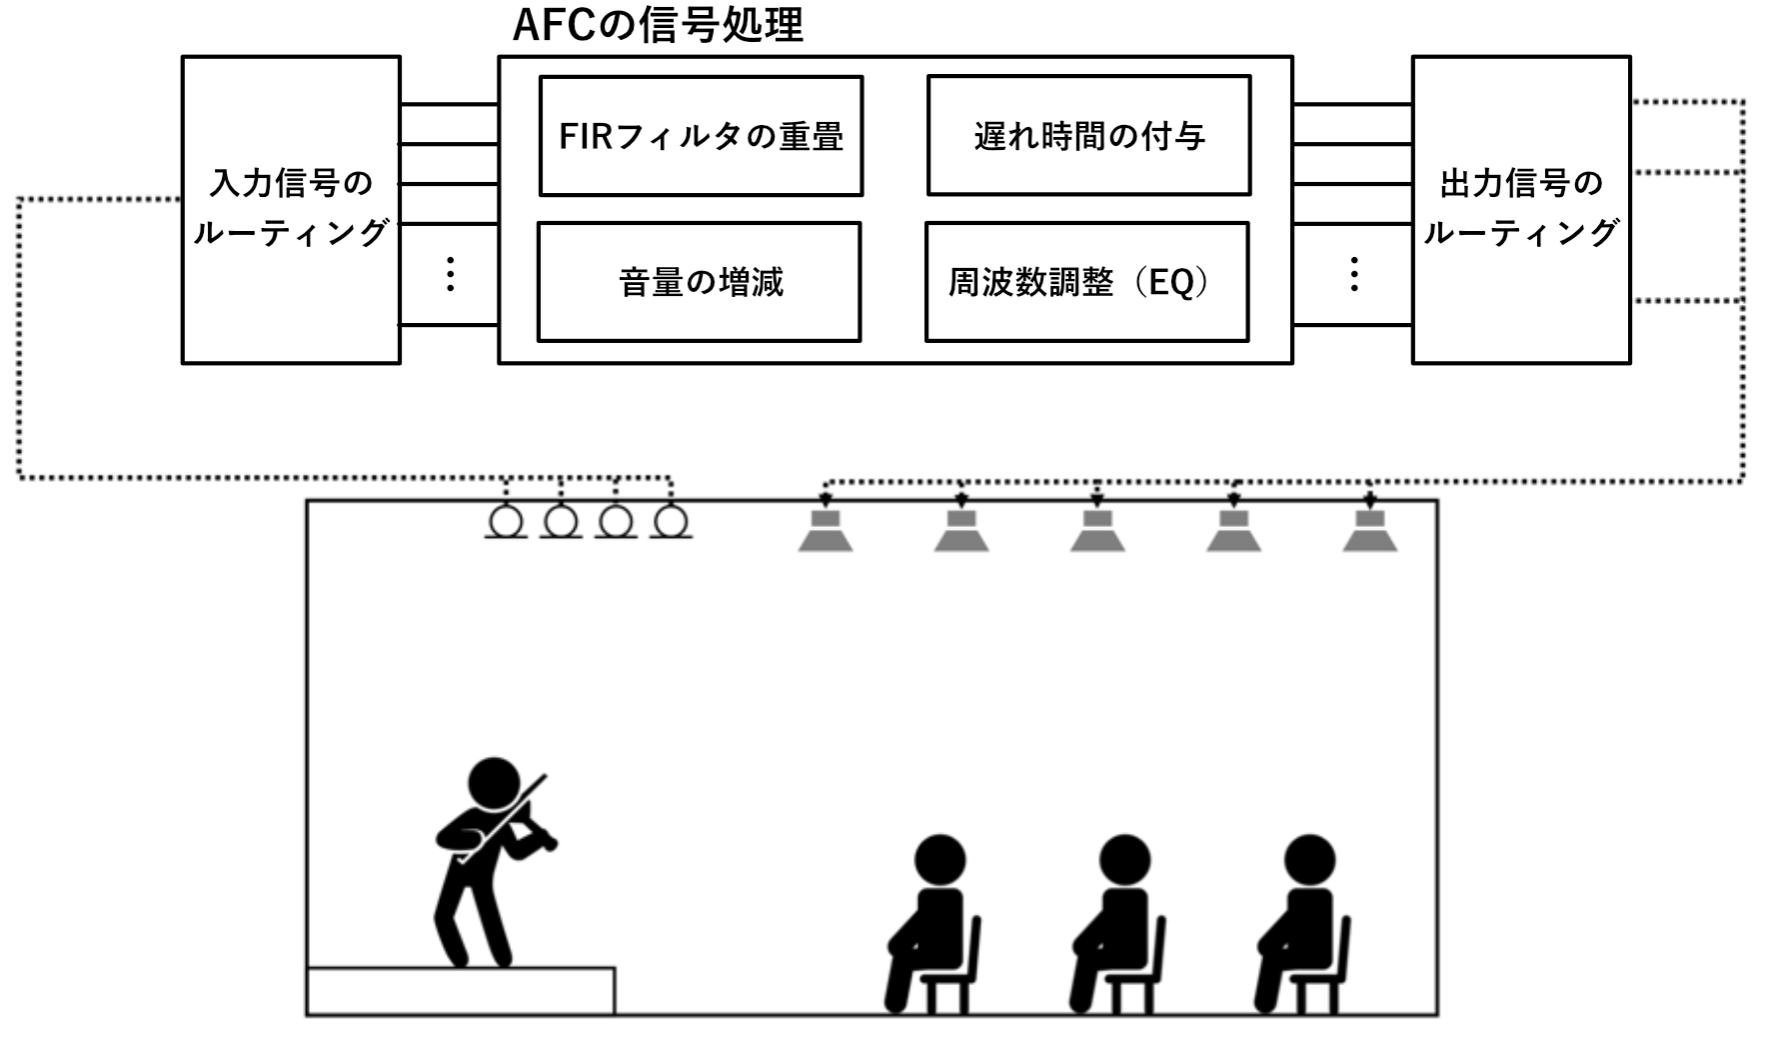
\includegraphics[width=0.9\linewidth]{images/AFCbusProcessing.png}
  \caption{busごとの信号処理の概要}
  \label{fig:busごとの信号処理の概要}
\end{figure}

\vspace*{\stretch{1}}

\begin{figure}[H]
  \centering
  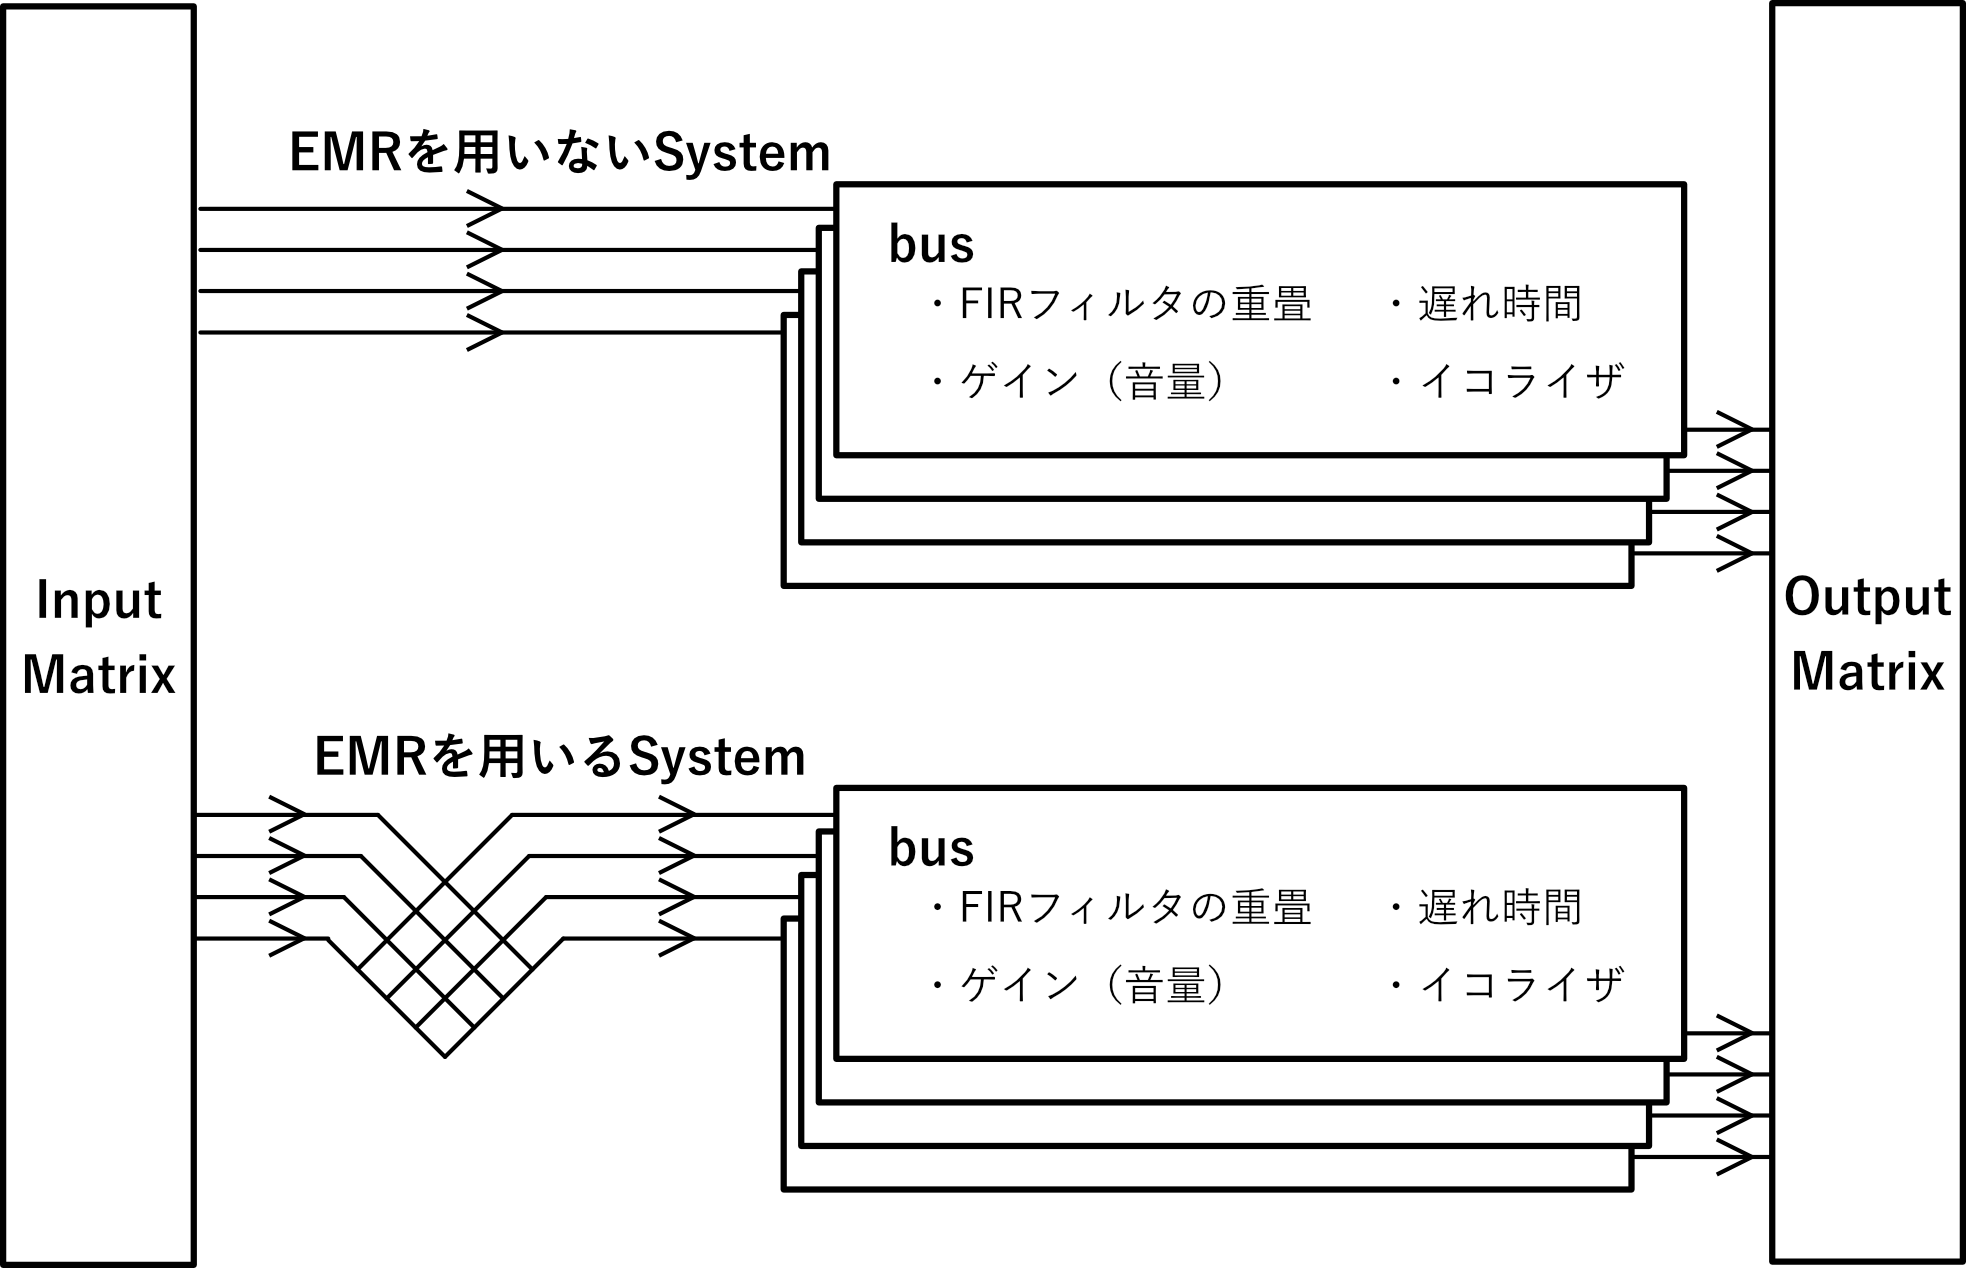
\includegraphics[width=0.9\linewidth]{images/AFCsystemProcessing.png}
  \caption{Systemによる信号処理の概要}
  \label{fig:Systemによる信号処理の概要}
\end{figure}

\vspace*{\stretch{1}}
%=======================================================================

\newpage
\subsection*{実験室におけるAFCのシステム機器配置}
もともとの響きの小さい室でAFCを用いることにより、大きな制御幅を得て自由度の高い音場の生成を行えることが期待できるため、本実験では半無響室にAFCを導入して用いることとした。導入したAFCシステムを構成する音響機材は4つのカージオイドマイク、4つの無指向性マイク、および20個のスピーカーであり、実験室の内部の様子を図\ref{fig:実験室の内部の様子}に、音響機材の配置を図\ref{fig:AFCのシステム機器配置}に示す。

また、生成する音場の評価を行うための音響測定は実験室の中央で行うものとし、音響測定時の測定機器の配置を図\ref{fig:音響測定機器の配置}に、そのときの様子を図\ref{fig:音響測定時の様子}示す。なお、紙面の上方を実験室の前方として実験室内における方向を定義した。

\vspace{\stretch{1}}
\begin{figure}[H]
  \centering
  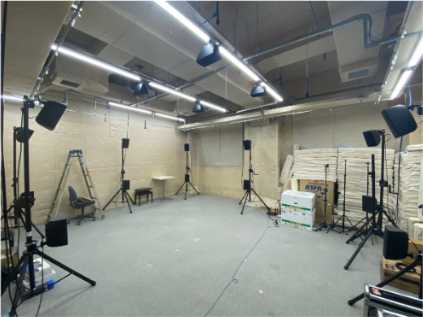
\includegraphics[width=0.6\linewidth]{images/twoPiRoom/twoPiRoomPhoto.png}
  \caption{実験室の内部の様子}
  \label{fig:実験室の内部の様子}
\end{figure}

\begin{figure}[H]
  \begin{minipage}[b]{0.5\linewidth}
    \centering
    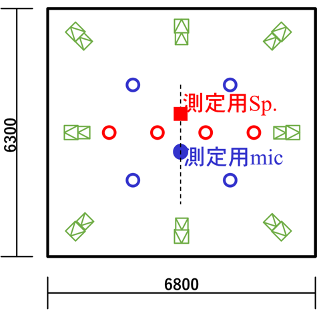
\includegraphics[width=.9\linewidth]{images/twoPiRoom/measureSetting.png}
    \caption{音響測定機器の配置}
    \label{fig:音響測定機器の配置}
  \end{minipage}%
  \begin{minipage}[b]{0.5\linewidth}
    \centering
    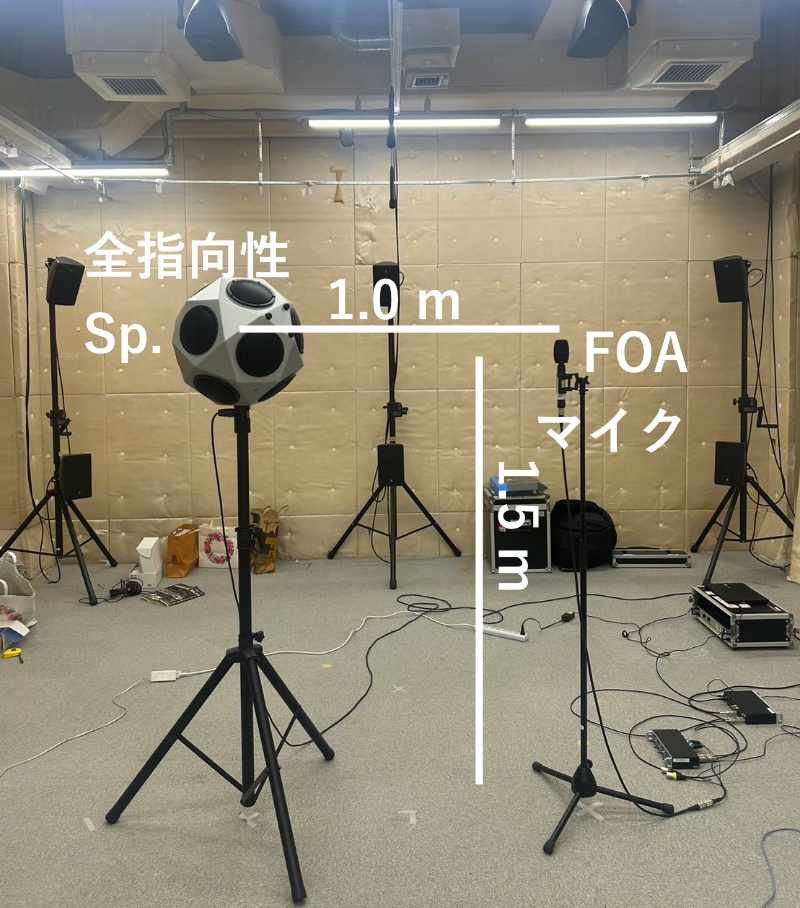
\includegraphics[width=.9\linewidth]{images/twoPiRoom/measureSettingPhotoResized.jpg}
    \caption{音響測定時の様子}
    \label{fig:音響測定時の様子}
  \end{minipage}
\end{figure}

\vspace{\stretch{1}}
%=======================================================================

\newpage
\vspace*{\stretch{1}}
\begin{figure}[H]
  \begin{minipage}[b]{1\linewidth}
    \centering
    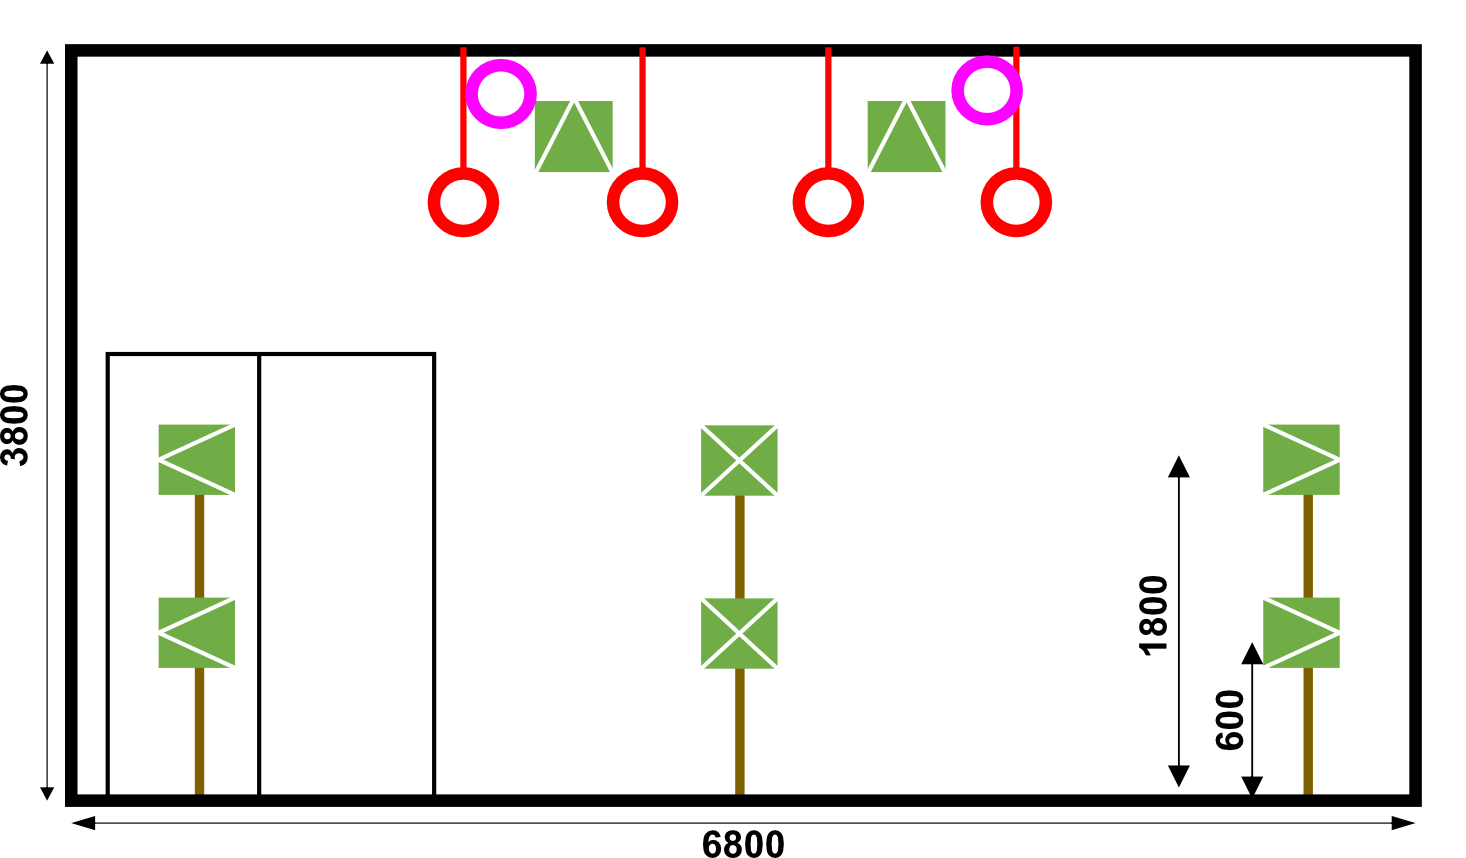
\includegraphics[width=.6\linewidth]{images/twoPiRoom/afcEquipArrayVertical.png}
    \subcaption{断面図}
    \label{fig:AFC機器配置断面図}
  \end{minipage}

  \begin{minipage}[b]{0.5\linewidth}
    \centering
    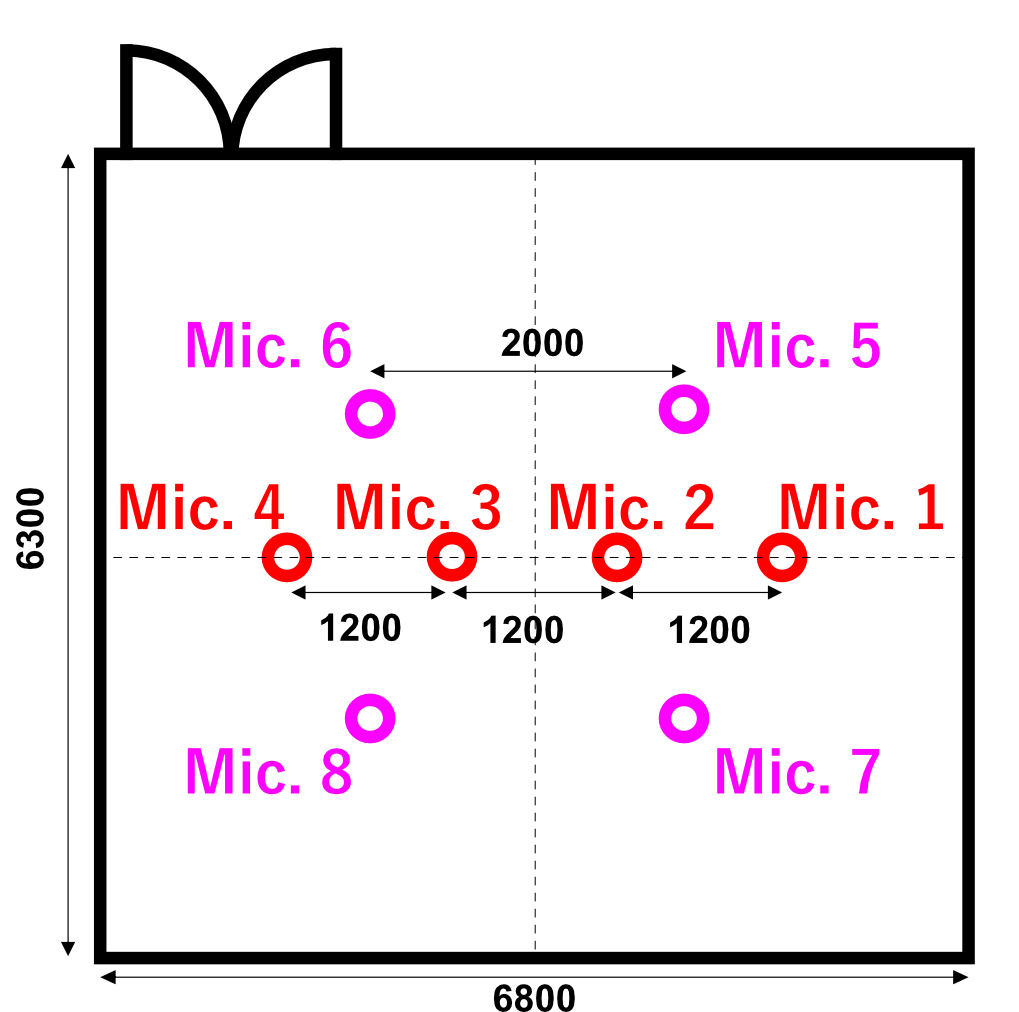
\includegraphics[width=.9\linewidth]{images/twoPiRoom/afcEquipArrayMic.png}
    \subcaption{マイクロホン配置}
    \label{fig:マイクロホン配置}
  \end{minipage}%
  \begin{minipage}[b]{0.5\linewidth}
    \centering
    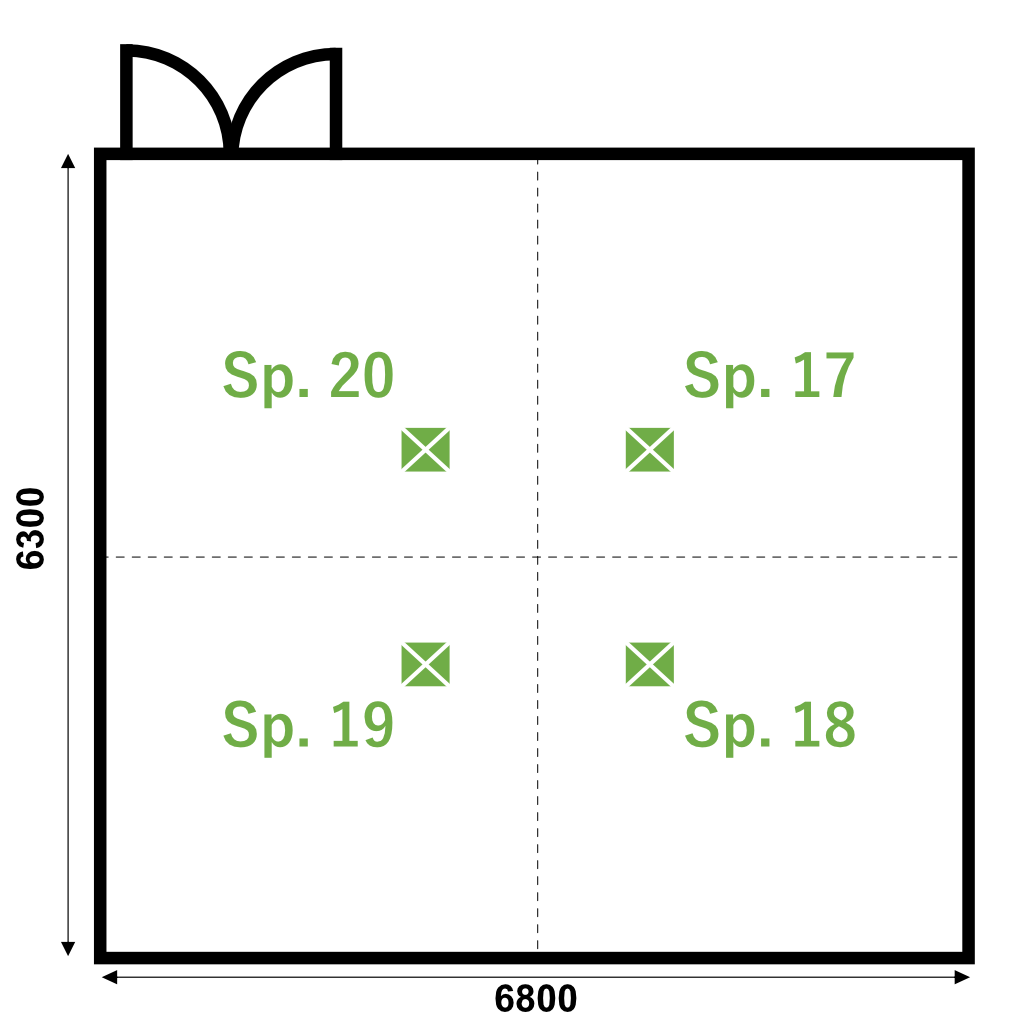
\includegraphics[width=.9\linewidth]{images/twoPiRoom/afcEquipArraySp3.png}
    \subcaption{スピーカー配置 三層目}
    \label{fig:スピーカー配置 三層目}
    \vfill
  \end{minipage}

  \begin{minipage}[b]{0.5\linewidth}
    \centering
    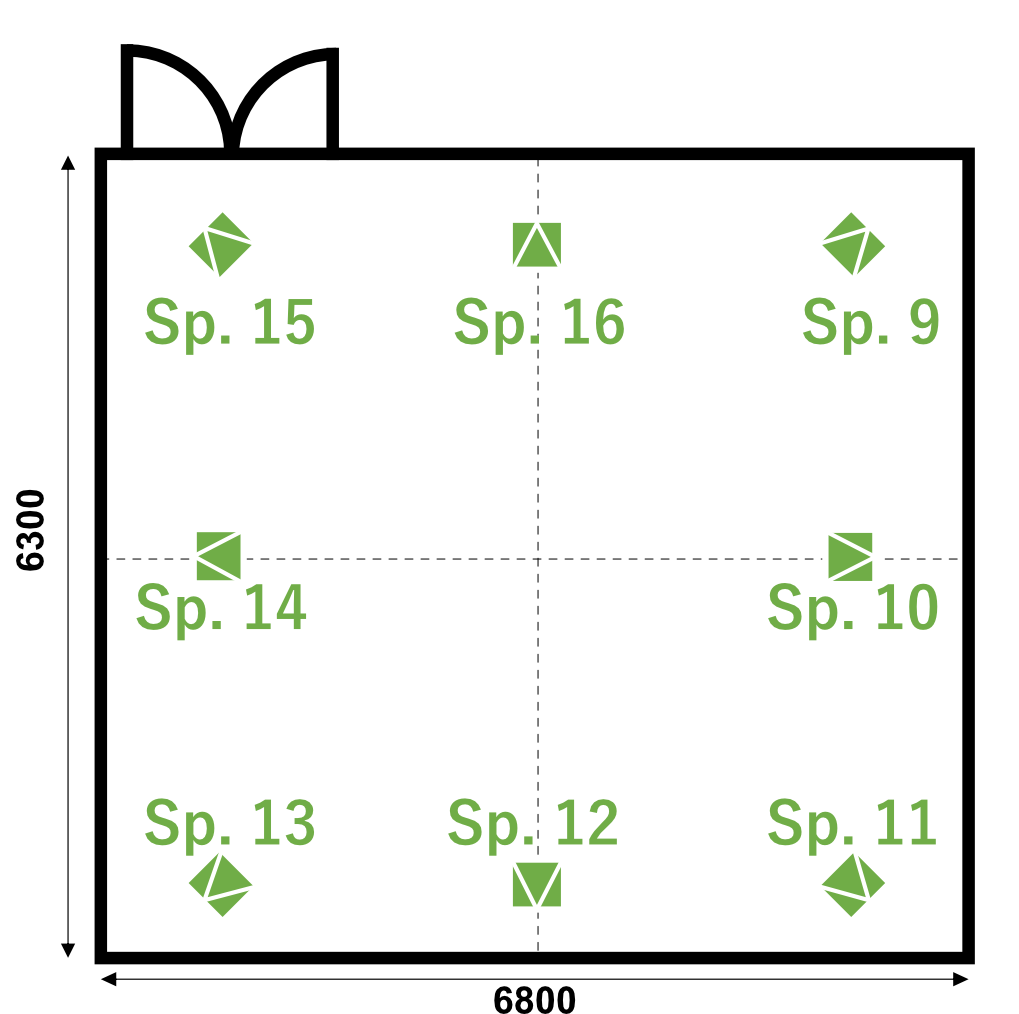
\includegraphics[width=.9\linewidth]{images/twoPiRoom/afcEquipArraySp2.png}
    \subcaption{スピーカー配置 二層目}
    \label{fig:スピーカー配置 二層目}
  \end{minipage}%
  \begin{minipage}[b]{0.5\linewidth}
    \centering
    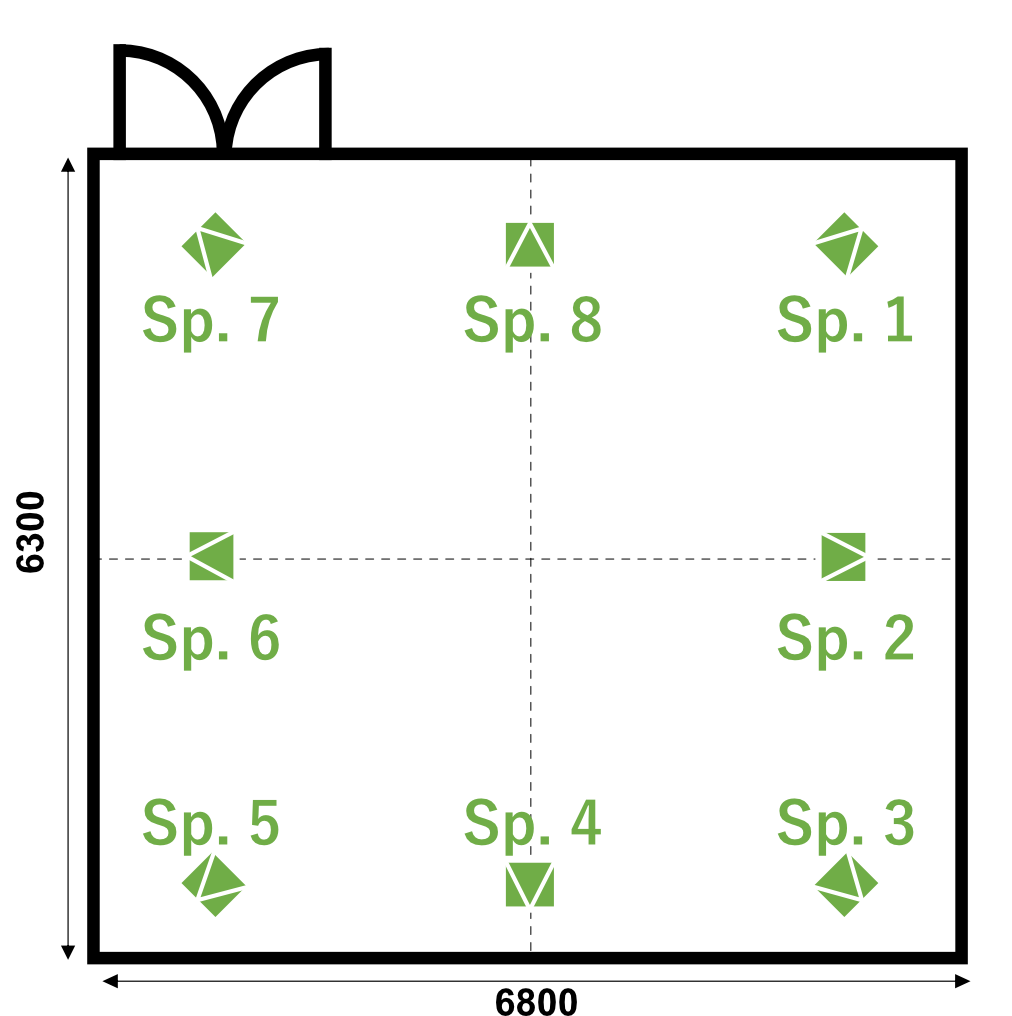
\includegraphics[width=.9\linewidth]{images/twoPiRoom/afcEquipArraySp1.png}
    \subcaption{スピーカー配置 一層目}
    \label{fig:スピーカー配置 一層目}
    \vfill
  \end{minipage}

  \caption{AFCのシステム機器配置}
  \label{fig:AFCのシステム機器配置}
\end{figure}
\vspace{\stretch{1}}

%=======================================================================
%\newpage
\section{音場の生成方法}
前節にてAFCシステムの仕組みと本研究で用いる実験室およびシステム機器構成について紹介した。本節では、AFCを用いた音場の生成方法について述べる。

\subsection*{マイクとスピーカーのルーティング}
2章4節にて設定した目標値を踏まえて、まず音場生成時のマイクとスピーカーのルーティングを決定する。前節で示したように、AFCのマイク入力はbusと呼ばれる信号処理系に割り当てられ、さらに4つのbusを一つのSystemとして取り扱う。本研究では、5つのSystemを作成して音場の生成を行った。

System1は、大まかな初期反射音成分の付加のため、入力系としてカージオイドマイクであるMic.1〜4の信号を用い、出力系として後方側からの再生音がやや多くなるように全方向のスピーカーを割り当てた。

System2は、水平面内からの全体的な後期反射音を満遍なく付加するため、マイクの入力とbusのルーティングを切り替える処理であるEMRをオンにした上で、入力系として全指向性マイクであるMic.5〜8の信号を用い、出力系として実験室の対角線上に配置した8つのスピーカーを割り当てた。

System3は、System2のみでは不足する上方からの後期反射音を増強して供給するため、入力系として全指向性マイクであるMic.5〜8の信号を用い、出力系として実験室の天井に設置した4つのスピーカーを割り当てた。

System4は、System1ではエネルギーの量が不足する後方からの初期反射音を増強しつつ、System1で小さくなるように調整する前方から初期反射音の供給量を細かく調整できるよう、出力系として実験室の後方に設置した3つのスピーカーと、前方に設置した1つのスピーカーを割り当てた。入力系としては、カージオイドマイクであるMic.1〜4を用いた場合にカラレーションが発生したため、全指向性マイクであるMic.5〜8の信号を用いた。

System5は、後期反射音の制御系だが、EMRの利用による後期反射音の方向特性の時変的な変化を是正して安定させるため、EMRの利用によるルーティングの切り替えは行わずに、全指向性マイクであるMic.5〜8の信号を用い、出力系として実験室の前後左右方向に設置した4つのスピーカーを割り当てた。

初期反射音および後期反射音ともに、床からの反射音供給によって、上方よりも下方からの寄与が大きくなる傾向が見られたため、System4およびSystem5では、前後左右方向の反射音供給を行うスピーカーとして、床面に近い1層目ではなく、床面から離れた2層目のスピーカーを用いた。

これらのルーティングを表\ref{tab:マイクとスピーカーのルーティング}に示す。

\newpage
\vspace*{\stretch{1}}
\begin{table}[H]
  \centering
  \caption{マイクとスピーカーのルーティング}
  \label{tab:マイクとスピーカーのルーティング}
  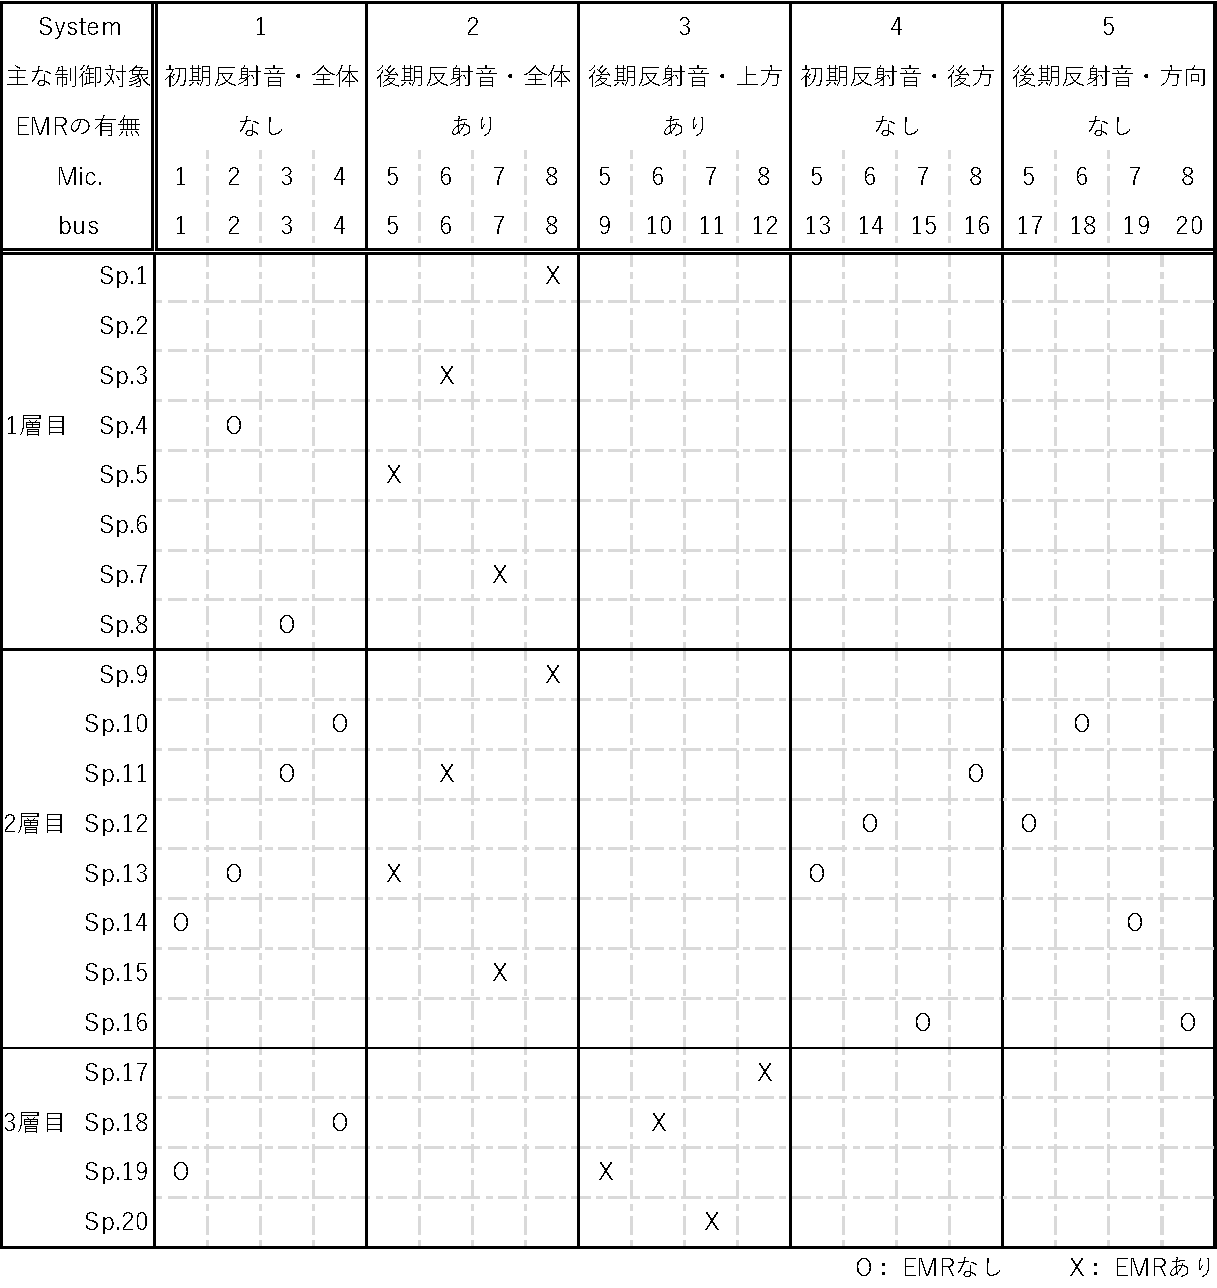
\includegraphics[width=1\linewidth]{images/experimentField/micSpRooting.pdf}
\end{table}
\vspace*{\stretch{1}}

%=======================================================================

\newpage
\subsection*{AFCの音場生成における制御幅}
実験室に響きを付加するにあたり、目標とした音場が実験室で実現可能な響きの幅、すなわち最小の響きの条件と最大の響きの範囲に収まることを確認する必要がある。

AFCは響きを増幅するシステムであるため、実験室で実現可能な最小の響きは、AFCをオフにしたときの響きとなる。AFCをオフししたときの$\mathrm{ST_{Early,dir}}$、$\mathrm{ST_{Late,dir}}$を表\ref{table:響き小の方向別ST}に示す。

この結果、AFCをオフにしたときの$\mathrm{ST_{Late,dir}}$は非常に小さく、この評価区間では音がほぼ完全に吸音されており、後期反射音についてはシステムで付加する成分によってほぼ完全に決定されると考えられる。一方で、$\mathrm{ST_{Early,dir}}$は$\SI{-25}{\dB}$前後と、$\mathrm{ST_{Late,dir}}$に比べて大きな値となっていた。これは半無響室に配置した吸音材に吸音され切らなかった低次の反射音がわずかに$100$〜$\SI{100}{\ms}$の間に残っているためと考えられる。特にFront方向では図\ref{fig:生成音場の目標値}に示した基準音場の生成目標値との差が約$\SI{3}{\dB}$に迫っており、慎重な調整が必要となる。

響きを増やすことに関してはある程度自由度を持って調整することができるが、AFCでつける響きを大きくしていく、つまり再生音の音量を上げていくと、ある音量を超えたときに不自然な音色の変化(カラレーション)が発生し始める。カラレーションが起こり始める音量の条件はイコライザの設定による周波数特性の変化をはじめとする様々な要素によって変化し、最大の響きの条件を厳密に調べることはできないが、イコライザによる周波数特性の補正を行わずに、その分のゲインの稼得を残す安全側にて響きの可変幅を大まかに検討する。周波数特性の手動調整を行わずに仮の設定でAFCをオンにして、カラレーションの生じ始めを聴感的に確認し、その直前の音量の設定における$\mathrm{ST_{Early,dir}}$および$\mathrm{ST_{Late,dir}}$を測定した。その結果を表\ref{table:響き大の方向別ST}に示す。

これらの結果から、実験室における$\mathrm{ST_{Early,dir}}$と$\mathrm{ST_{Late,dir}}$はコンサートホールでの実測値と同程度の値を十分取ることができると考えられ、詳細な設定により所望の音場を実現しうることが期待できる。

\vspace{\stretch{1}}
\begin{table}[H]
  \centering
  \caption{AFCをオフにしたときの$\mathrm{ST_{Early,dir}}$、$\mathrm{ST_{Late,dir}}$}
  \label{table:響き小の方向別ST}
  \begin{tabular}{c|cccccc} \hline \hline
    \begin{tabular}{c}
    
    \end{tabular}&
    \begin{tabular}{c}
      Front
    \end{tabular}&
    \begin{tabular}{c}
      Back
    \end{tabular}&
    \begin{tabular}{c}
      Left
    \end{tabular}&
    \begin{tabular}{c}
      Right
    \end{tabular}&
    \begin{tabular}{c}
      Up
    \end{tabular}&
    \begin{tabular}{c}
      Down
    \end{tabular} \\ \hline
    $\mathrm{ST_{Early,dir}}$ (dB) & -24.2 & -25.5 & -24.2 & -25.9 &-25.9 & -23.3 \\
    $\mathrm{ST_{Late,dir}}$ (dB) & -65.5 & -66.7 & -67.0 &-65.6 & -66.6 & -64.2 \\ \hline \hline
  \end{tabular}
\end{table}

\begin{table}[H]
  \centering
  \caption{AFC仮調整時の$\mathrm{ST_{Early,dir}}$、$\mathrm{ST_{Late,dir}}$}
  \label{table:響き大の方向別ST}
  \begin{tabular}{c|cccccc} \hline \hline
    \begin{tabular}{c}
    
    \end{tabular}&
    \begin{tabular}{c}
      Front
    \end{tabular}&
    \begin{tabular}{c}
      Back
    \end{tabular}&
    \begin{tabular}{c}
      Left
    \end{tabular}&
    \begin{tabular}{c}
      Right
    \end{tabular}&
    \begin{tabular}{c}
      Up
    \end{tabular}&
    \begin{tabular}{c}
      Down
    \end{tabular} \\ \hline
    $\mathrm{ST_{Early,dir}}$ (dB) & -16.4 & -18.0 & -16.7 & -17.3 & -19.9 & -16.1\\
    $\mathrm{ST_{Late,dir}}$ (dB) & -15.8 & -15.9 & -16.0 & -15.8 & -19.2 & -15.0\\ \hline \hline
  \end{tabular}
\end{table}

\vspace{\stretch{1}}
%=======================================================================
\newpage
    

%=====================================================================================

  \section{生成音場の調整方法}
    
    \subsection{方向別STの調整方法}
    実測した方向別STの値をもとに、生成する音場の方向別STを調整する。$\mathrm{ST_{Early,dir}}$は後方が大きく、
    $\mathrm{ST_{Late,dir}}$は全方向から満遍なく反射音が到来していることがわかるため、このような方向特性を
    実現することができるようにマイクとスピーカーの配置と結線を行った。実験室のシステム機器配置を
    図\ref{fig:実験室におけるAFCのシステム機器配置}に、これらのルーティングを表\ref{tab:マイクとスピーカーのルーティング}に示す。
    

    また、響きの可変幅を十分に確保できるよう、重畳するFIRフィルタには図\ref{fig:FIRフィルタを測定したコンサートホール}に
    示す2000席程度の豊かな響きを持つコンサートホールにて実測したインパルス応答を用いた。初期反射音制御部には舞台付近で
    測定したインパルス応答を、後期反射音制御部には舞台から遠方にて測定したインパルス応答を用いた。それぞれについて、ともに
    異なる4点で測定したインパルス応答を用いており、これは完全に同じインパルス応答を用いることによってAFCシステム内の
    ループごとの周波数特性が近くなることでカラレーションに対する安定性が低下するのを防ぐことを目的としている。
    重畳に用いたインパルス応答の時間波形を図\ref{fig:初期反射音の重畳に用いたFIRフィルタ}および
    図\ref{fig:後期反射音の重畳に用いたフィルタ}に示す。

    \begin{figure}[H]
      \centering
      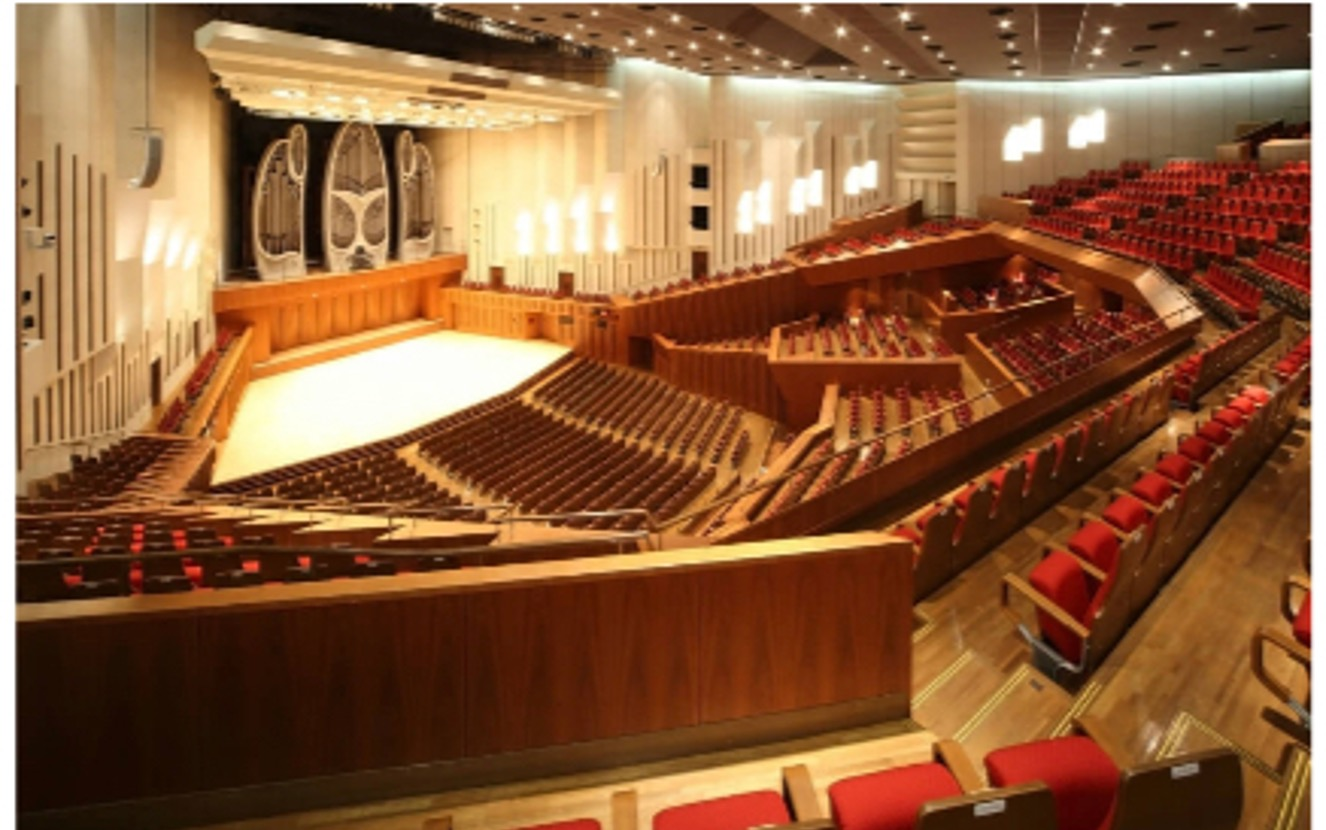
\includegraphics[width=.6\linewidth]{images/convolutedIrHall.jpg}
      \caption{FIRフィルタを測定したコンサートホール}
      \label{fig:FIRフィルタを測定したコンサートホール}
    \end{figure}

    \begin{figure}[H]
      \begin{minipage}[b]{.5\linewidth}
          \centering
          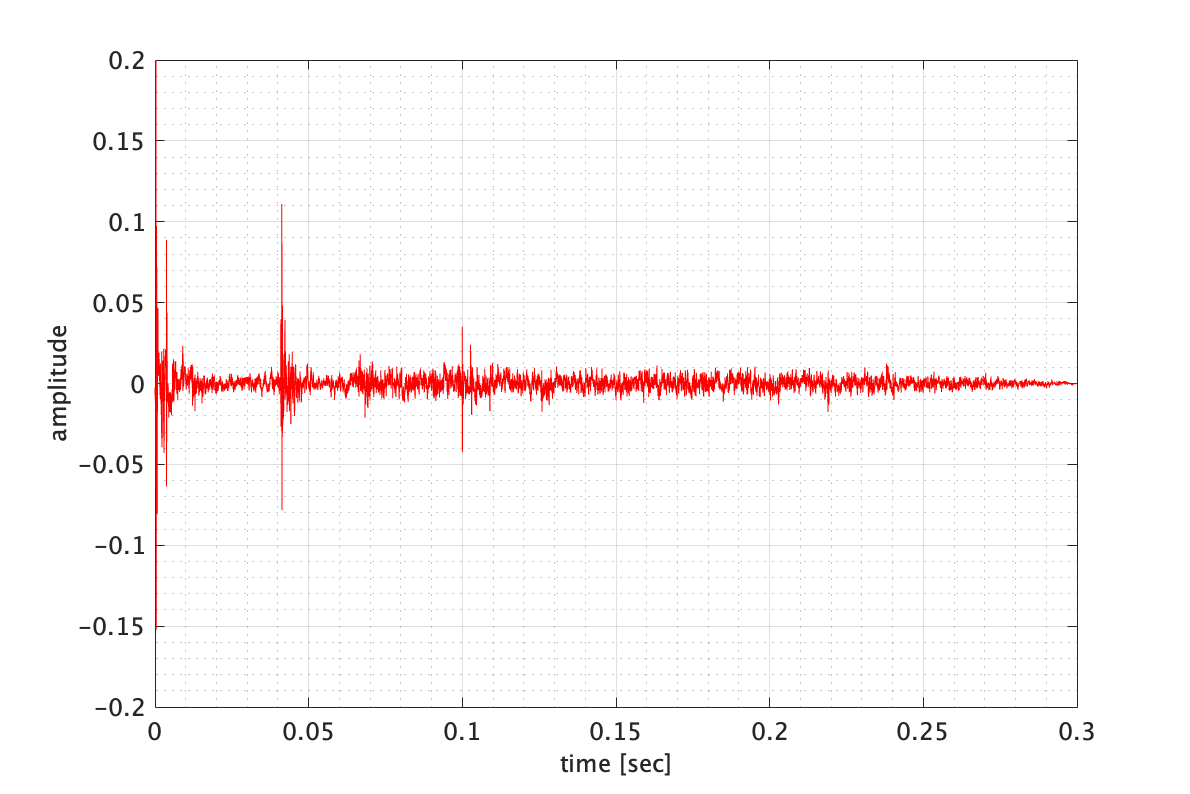
\includegraphics[width=.9\linewidth]{images/convolutedIr/ER1.png}
          \subcaption*{FIRフィルタ 1}
      \end{minipage}%
      \begin{minipage}[b]{.5\linewidth}
          \centering
          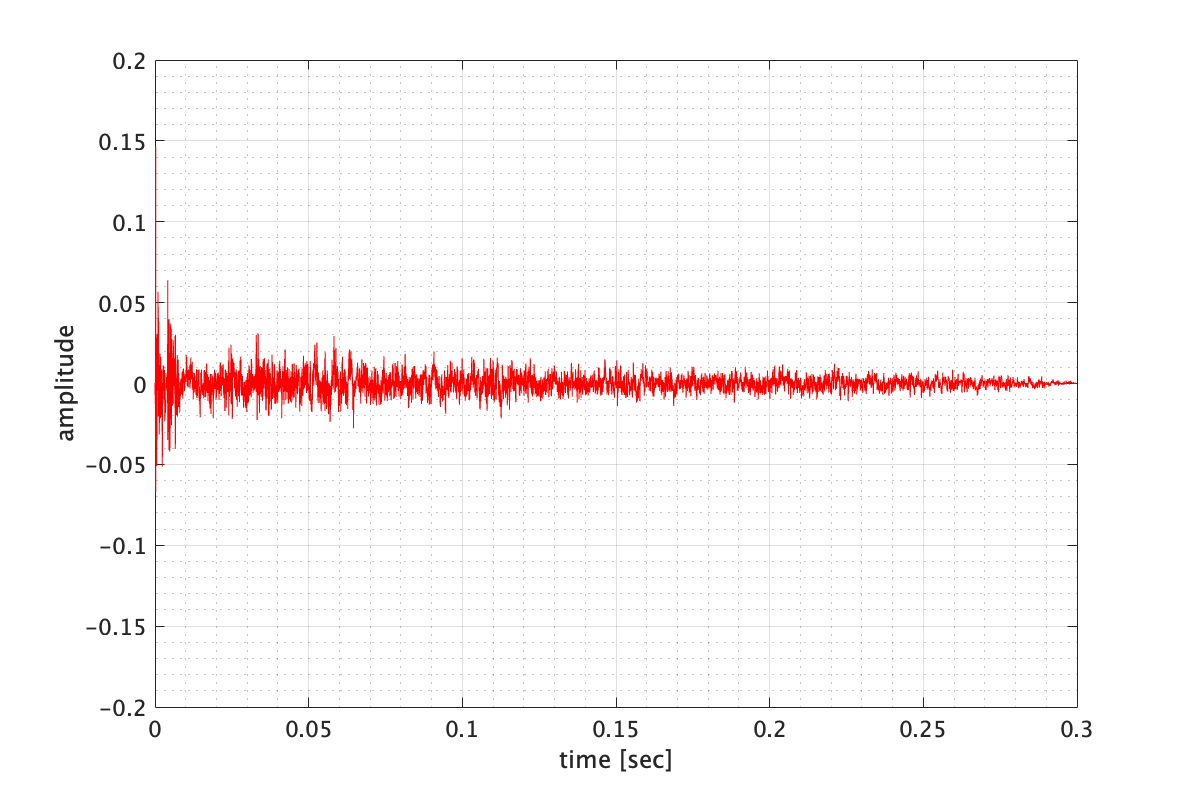
\includegraphics[width=.9\linewidth]{images/convolutedIr/ER2.png}
          \subcaption*{FIRフィルタ 2}
      \end{minipage}

      \begin{minipage}[b]{.5\linewidth}
          \centering
          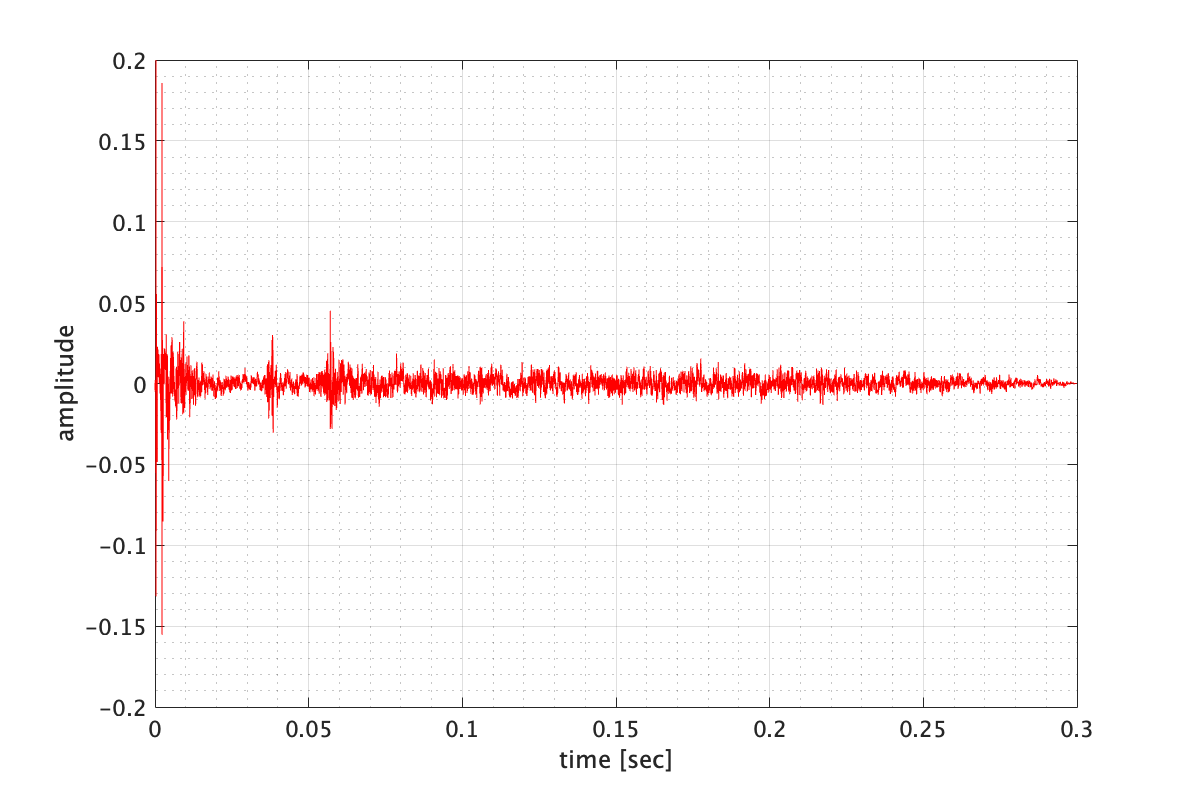
\includegraphics[width=.9\linewidth]{images/convolutedIr/ER3.png}
          \subcaption*{FIRフィルタ 3}
      \end{minipage}%
      \begin{minipage}[b]{.5\linewidth}
          \centering
          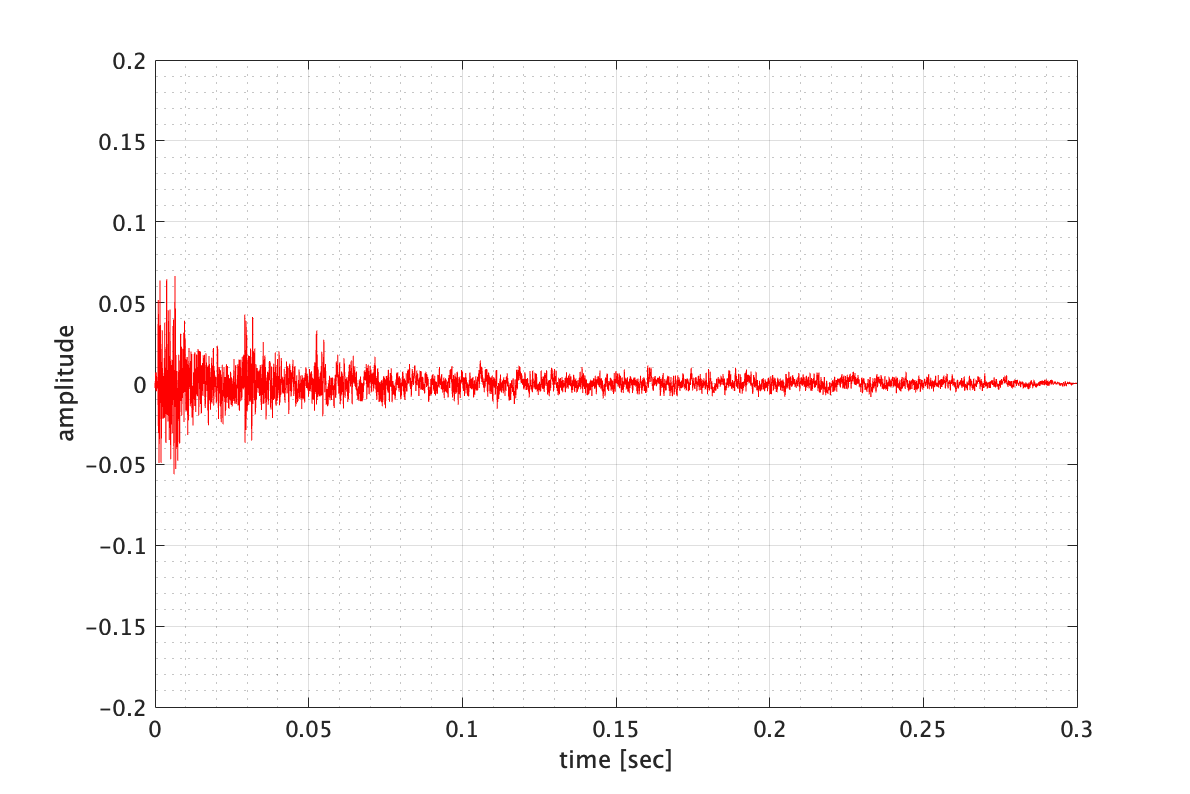
\includegraphics[width=.9\linewidth]{images/convolutedIr/ER4.png}
          \subcaption*{FIRフィルタ 4}
      \end{minipage}

      \centering
      \caption{初期反射音の重畳に用いたFIRフィルタ}
      \label{fig:初期反射音の重畳に用いたFIRフィルタ}
    \end{figure}

    \begin{figure}[H]
      \begin{minipage}[b]{.5\linewidth}
          \centering
          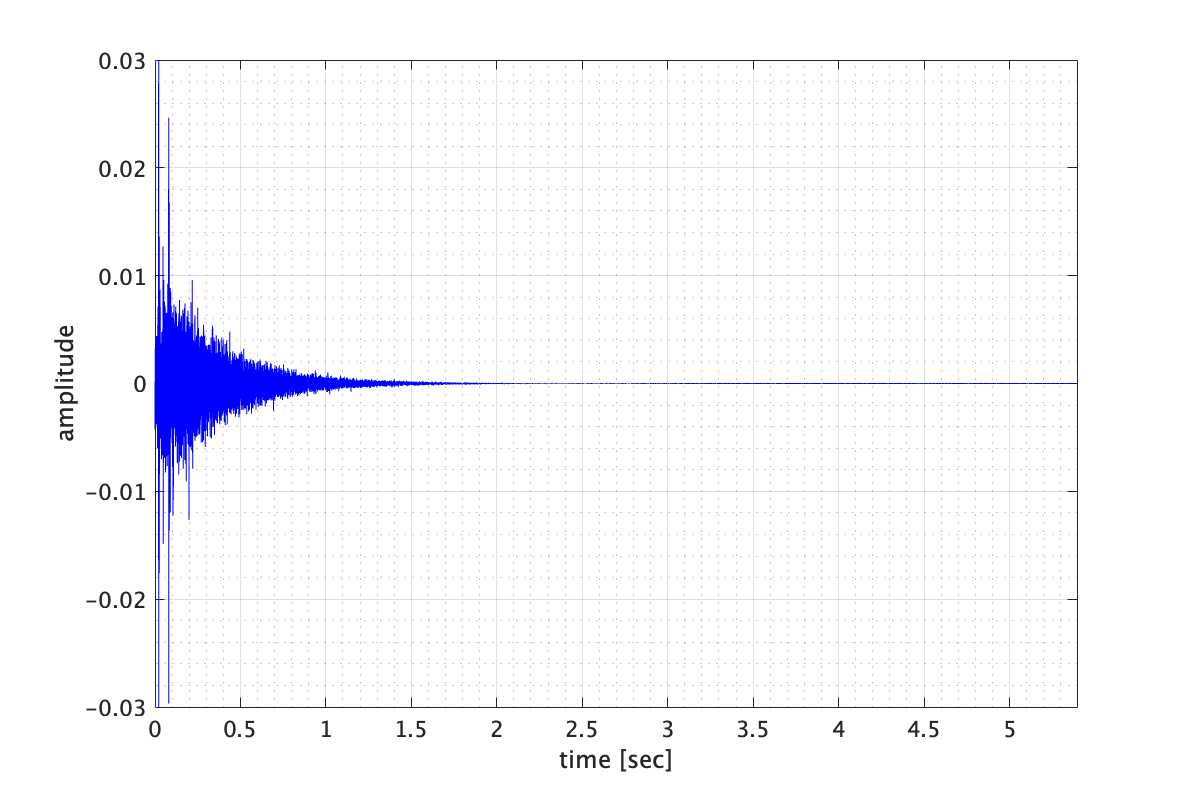
\includegraphics[width=.9\linewidth]{images/convolutedIr/REV1.png}
          \subcaption*{FIRフィルタ 1}
      \end{minipage}%
      \begin{minipage}[b]{.5\linewidth}
          \centering
          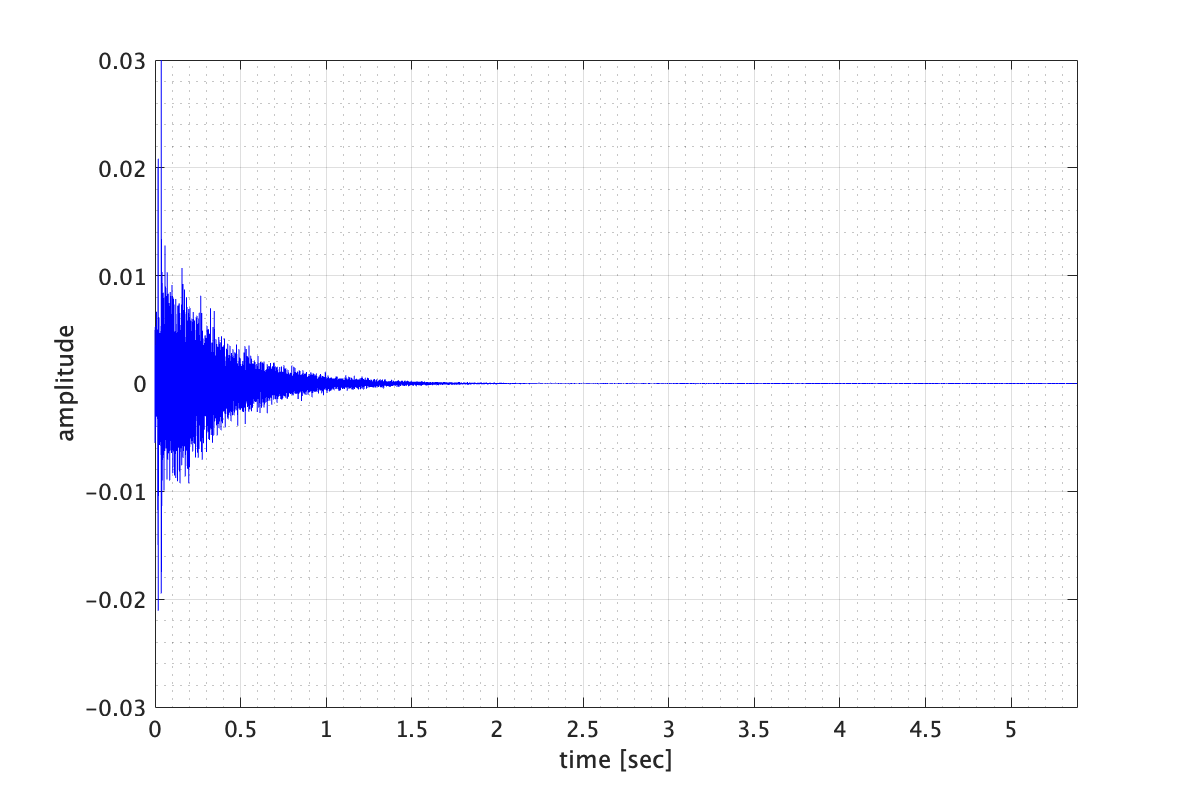
\includegraphics[width=.9\linewidth]{images/convolutedIr/REV2.png}
          \subcaption*{FIRフィルタ 2}
      \end{minipage}

      \begin{minipage}[b]{.5\linewidth}
          \centering
          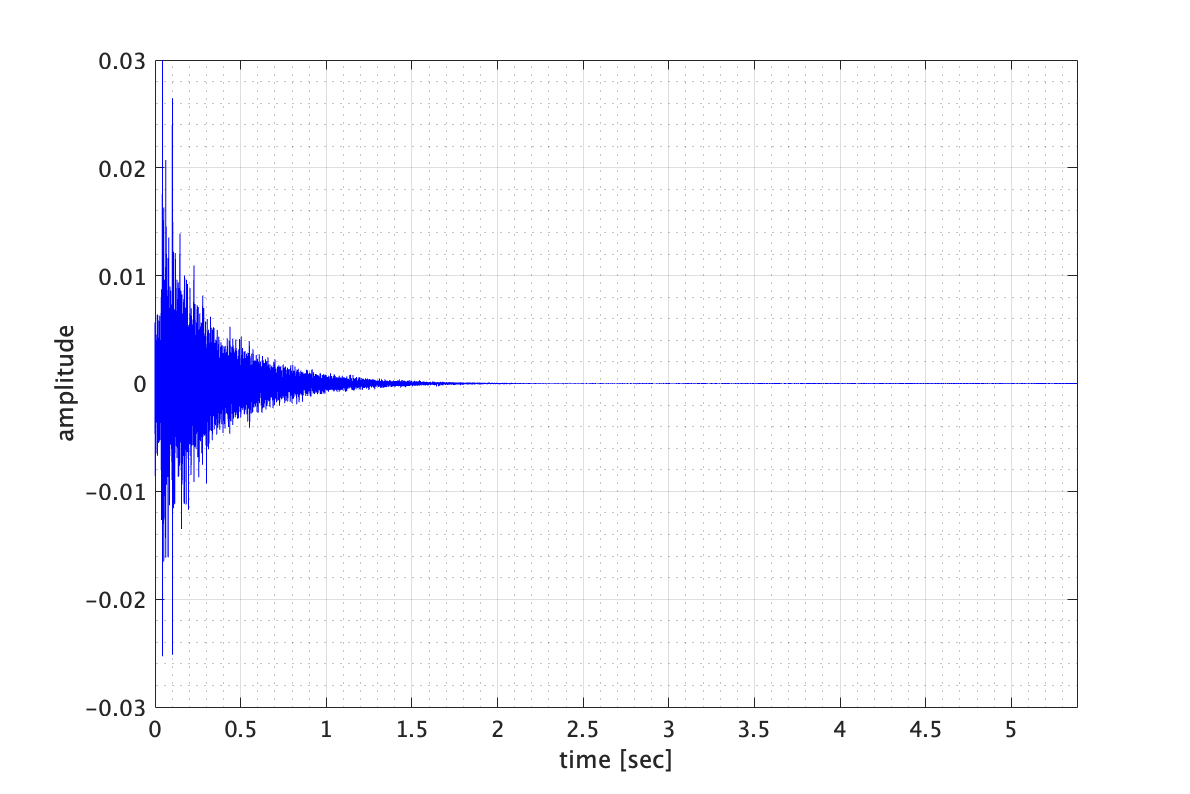
\includegraphics[width=.9\linewidth]{images/convolutedIr/REV3.png}
          \subcaption*{FIRフィルタ 3}
      \end{minipage}%
      \begin{minipage}[b]{.5\linewidth}
          \centering
          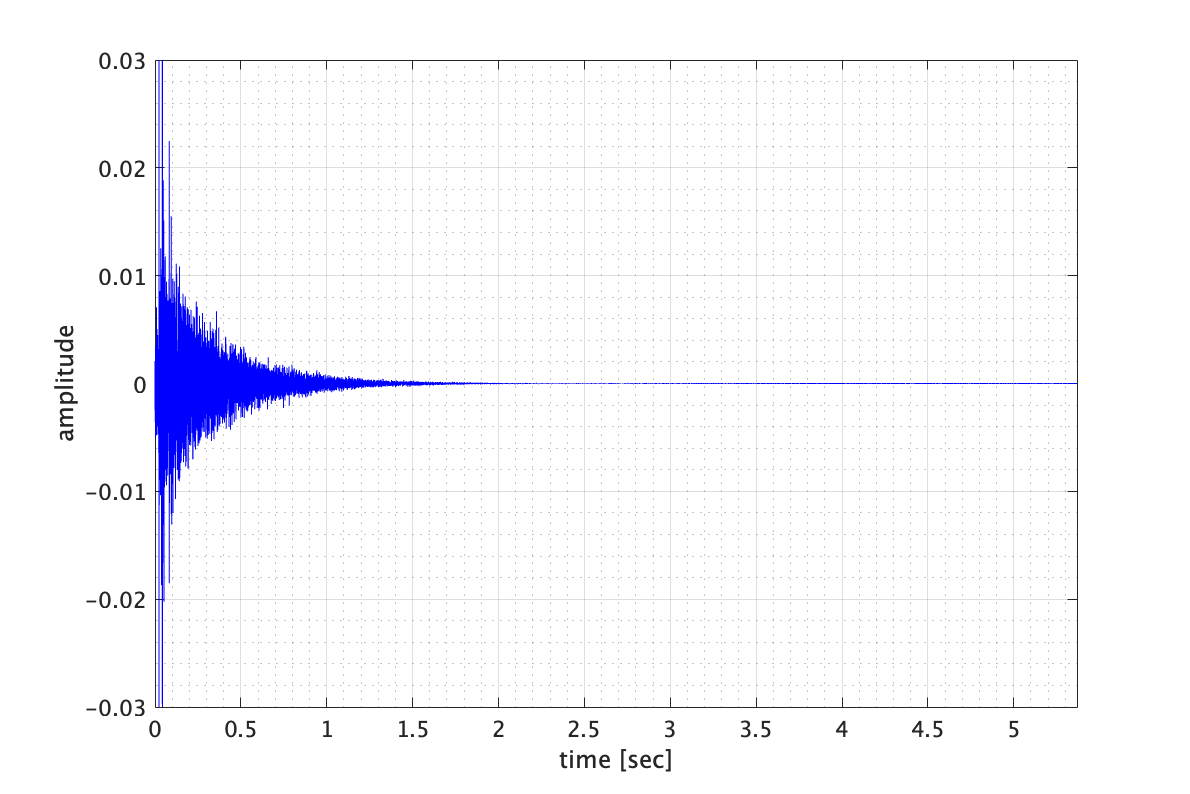
\includegraphics[width=.9\linewidth]{images/convolutedIr/REV4.png}
          \subcaption*{FIRフィルタ 4}
      \end{minipage}

      \centering
      \caption{後期反射音の重畳に用いたFIRフィルタ}
      \label{fig:後期反射音の重畳に用いたフィルタ}
    \end{figure}

    $\mathrm{ST_{Early,dir}}$および$\mathrm{ST_{Late,dir}}$を目標値に近づけて制御するためには、初期反射音と
    後期反射音の成分をある程度独立に制御することが必要となる。初期反射音制御部のために付加したエネルギーが後期反射音の
    評価区間に漏れ出す量を少なくするため、初期反射音制御部では重畳するFIRフィルタにフェードアウトを設定することにより
    信号長を$\SI{120}{ms}$に限定した。
    
    また、後期反射音制御部では、反射音の付加に長い遅れ時間を加えることで$\mathrm{ST_{Early,dir}}$の評価区間に入るエネルギーを
    減らすことができるが、遅れ時間が大きすぎるとエコー障害が生じる恐れがある。本研究では、$\SI{45}{ms}$の遅れ時間を
    付け加えることにより、聴感的な自然さを保ちつつ$\mathrm{ST_{Early,dir}}$への影響を低減した。

    \subsection{その他の音響特性の調整方法}
      \subsubsection{残響時間の調整}
      本実験で用いた実験室における音響測定では、部屋の広さによる制約により、直接音の減衰が大きいため残響時間の評価として
      よく用いられる $\mathrm{T_{20}}$ または $\mathrm{T_{30}}$ を適切に測定することができない。
      そこで本研究では、$\mathrm{ST}$の測定条件によるインパルス応答の測定結果からエネルギーの減衰曲線を描き、
      $\SI{-15}{dB}$から$\SI{-45}{dB}$までの減衰曲線の傾きを読むことにより残響時間を求めた。
      生成した音場の残響時間は通常よくあるコンサートホールでの残響時間よりもかなり長くなる傾向があったため、
      後期反射音制御部で重畳するFIRフィルタにフェードアウトを設定することで残響時間を短くし、$\SI{1.8}{秒}$程度
      の自然な長さになるよう調整した。
      
      \subsubsection{周波数特性の調整}
      オクターブバンドごとのSTおよび残響時間の値が極端にばらつくことを防ぐため、測定とAFCシステム内部の
      イコライザの調整を繰り返して周波数特性を調整した。

%=====================================================================================

\section{生成した音場の特性}

  \subsection{基準音場}
  コンサートホールのステージを模して生成した基準音場の方向別STを図\ref{fig:基準音場の方向別ST}に示す。
  各方向での目標値からの差はすべて$\SI{1}{dB}$未満であり、およそ目標値の通りの方向別STを実現することが
  できた。
  
  残響時間およびSTを図\ref{fig:基準音場の残響時間とST}に示す。残響時間および$\mathrm{ST_{Late,dir}}$は
  すべてのオクターブバンドでほぼフラットな周波数特性となった。$\mathrm{ST_{Early,dir}}$は室自体の持つ特性
  が影響していると考えられ、完全な制御はできていないが、平均値からの偏差はすべてのオクターブバンドで$\SI{1}{dB}$
  程度に収めることができた。
  
  減衰曲線を図\ref{fig:基準音場の減衰曲線}に示す。AFCで生成した音場では、エネルギーの付加によって特に響きの
  後期反射音側で減衰曲線が盛り上がる場合があるが、今回生成した音場ではこのような現象は見られず、実際の空間と
  同様の直線的な減衰が確認できた。

  \begin{figure}[H]
    \begin{minipage}
      [b]{.5\linewidth}
      \centering
      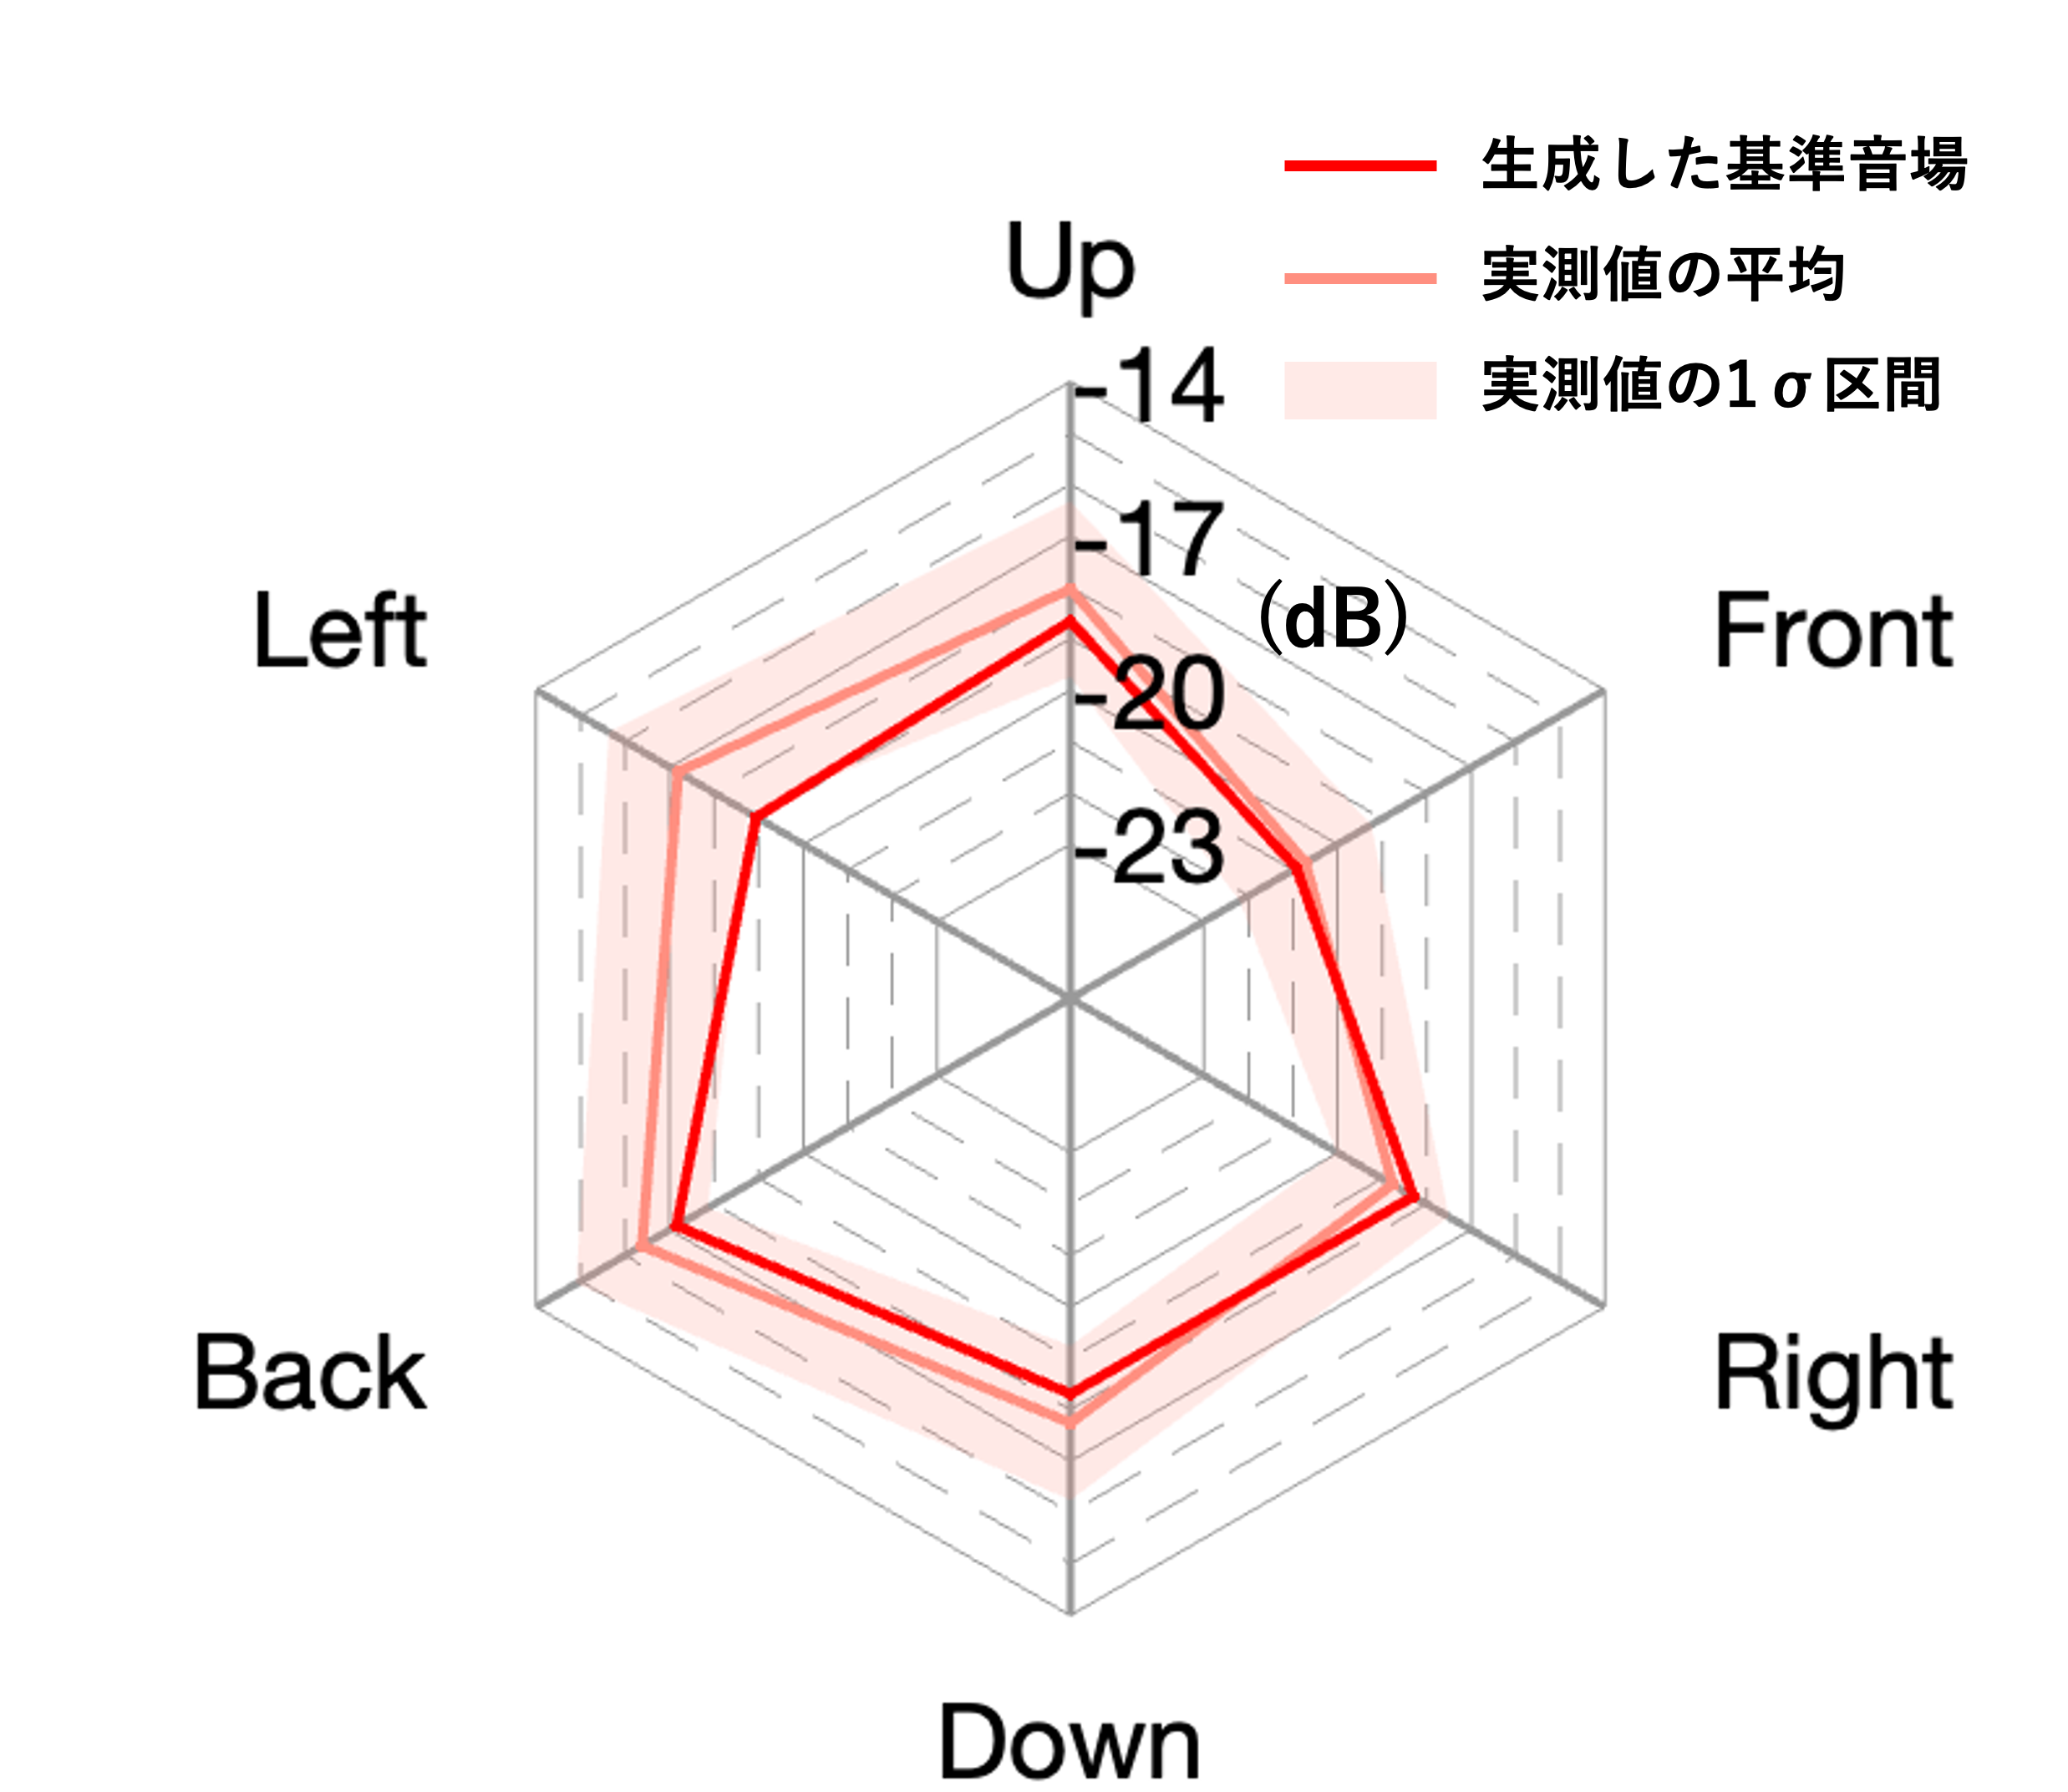
\includegraphics[width=1\linewidth]{images/experimentField/withLegend/baseEarlyOnTarget4.png}
      \subcaption*{$\mathrm{ST_{Early,dir}}$}
    \end{minipage}%
    \begin{minipage}
      [b]{.5\linewidth}
      \centering
      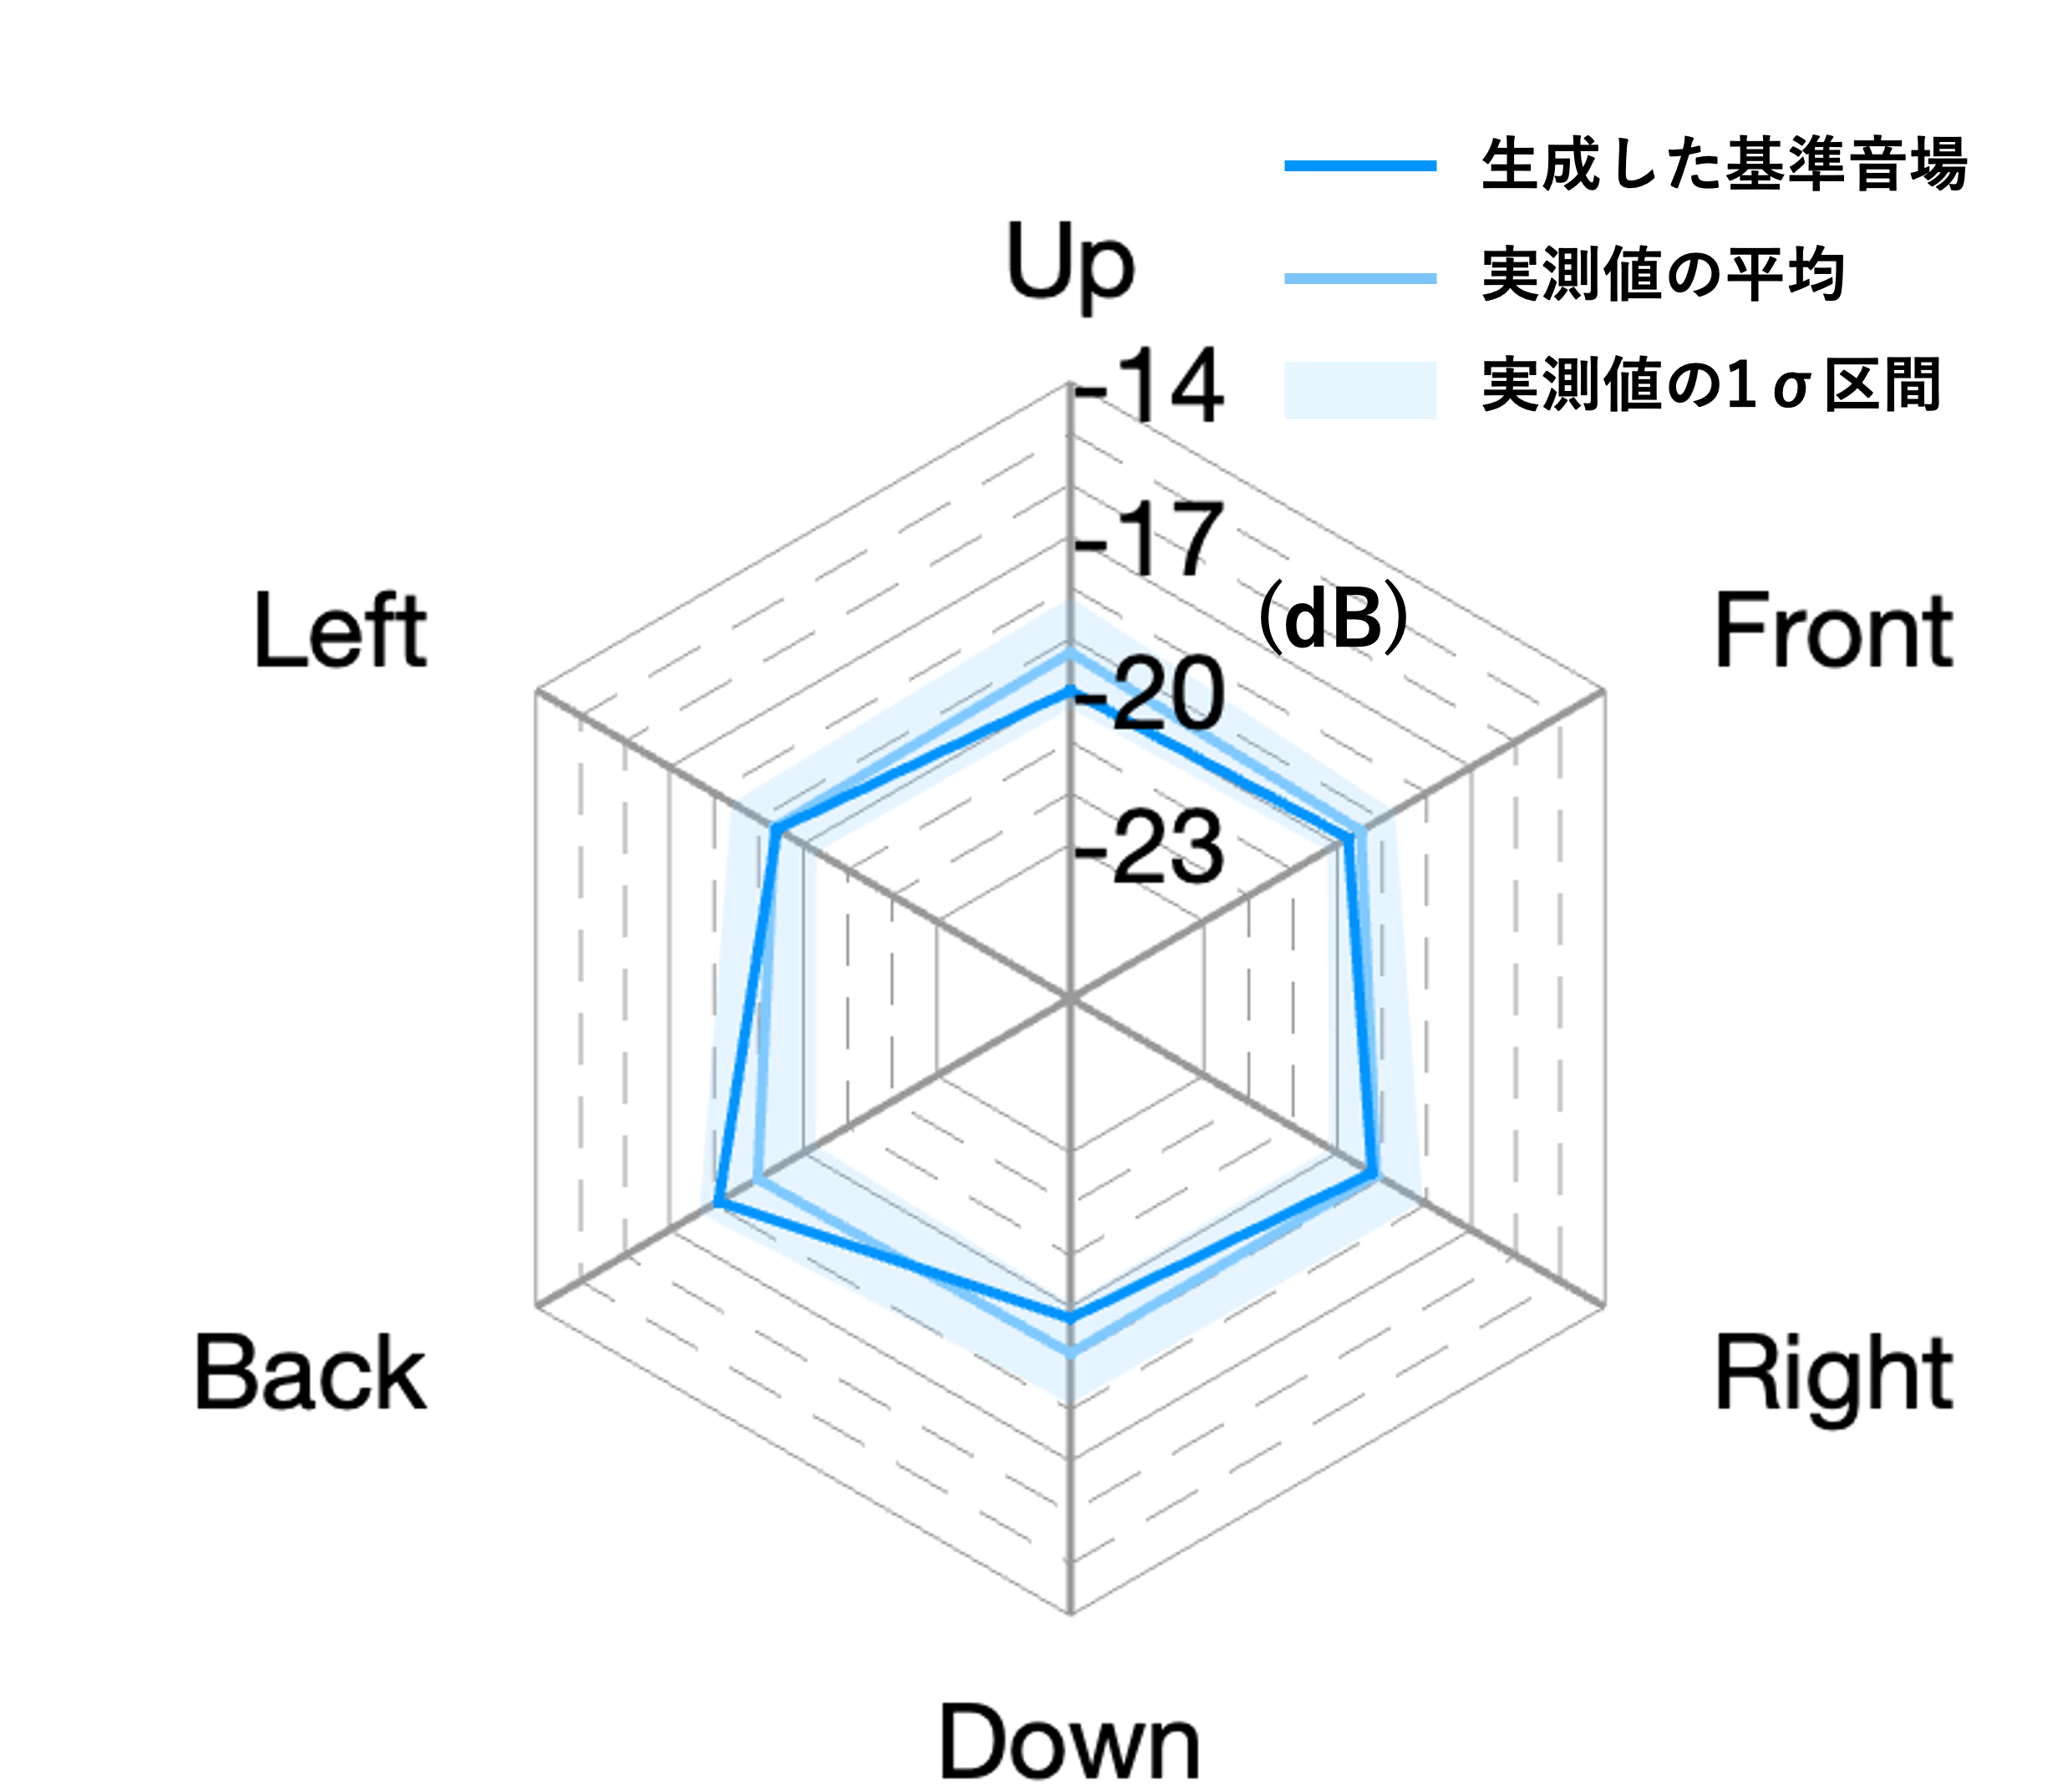
\includegraphics[width=1\linewidth]{images/experimentField/withLegend/baseLateOnTarget4.png}
      \subcaption*{$\mathrm{ST_{Late,dir}}$}
      \end{minipage}
    \caption{基準音場の方向別ST}
    \label{fig:基準音場の方向別ST}
  \end{figure}

  \begin{figure}[H]
    \centering
    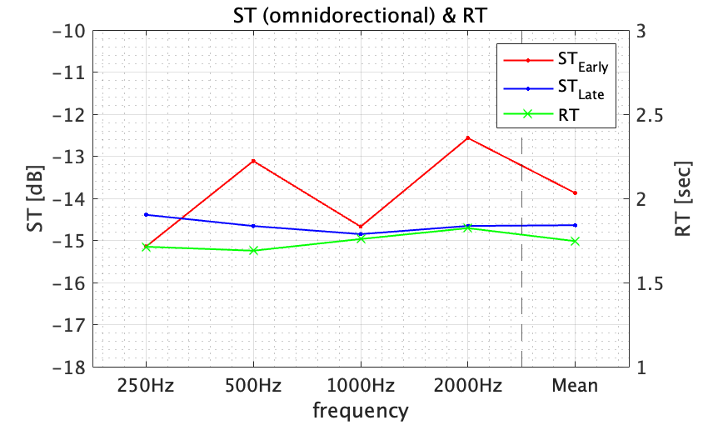
\includegraphics[width=.8\linewidth]{images/fieldO_stRt.png}
    \caption{基準音場の残響時間とST}
    \label{fig:基準音場の残響時間とST}
  \end{figure}

  \begin{figure}[H]
    \centering
    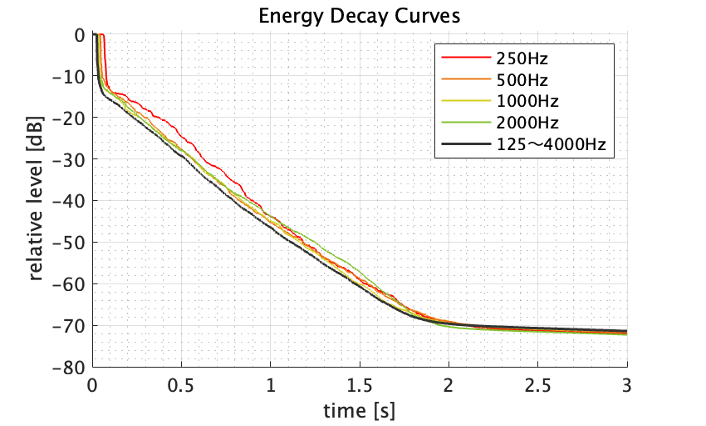
\includegraphics[width=.8\linewidth]{images/fieldO_EnergyDecayCurve.png}
    \caption{基準音場の減衰曲線}
    \label{fig:基準音場の減衰曲線}
  \end{figure}

  %=====================================================================================

  \subsection{方向の偏りをつけた音場}
  基準音場に対して、初期反射音・後期反射音のそれぞれについて、前方からの反射を強めた音場と後方からの反射を
  強めた音場を生成した。初期反射音の前方を強めた音場を音場A、初期反射音の後方を強めた音場を音場B、後期反射音の
  前方を強めた音場を音場C、後期反射音の後方を強めた音場を音場Dとする。生成した音場の方向別STを
  図\ref{fig:音場Aの方向別ST}から図\ref{fig:音場Dの方向別ST}に示す。

  \begin{figure}[H]
    \begin{minipage}[b]{.5\linewidth}
        \centering
        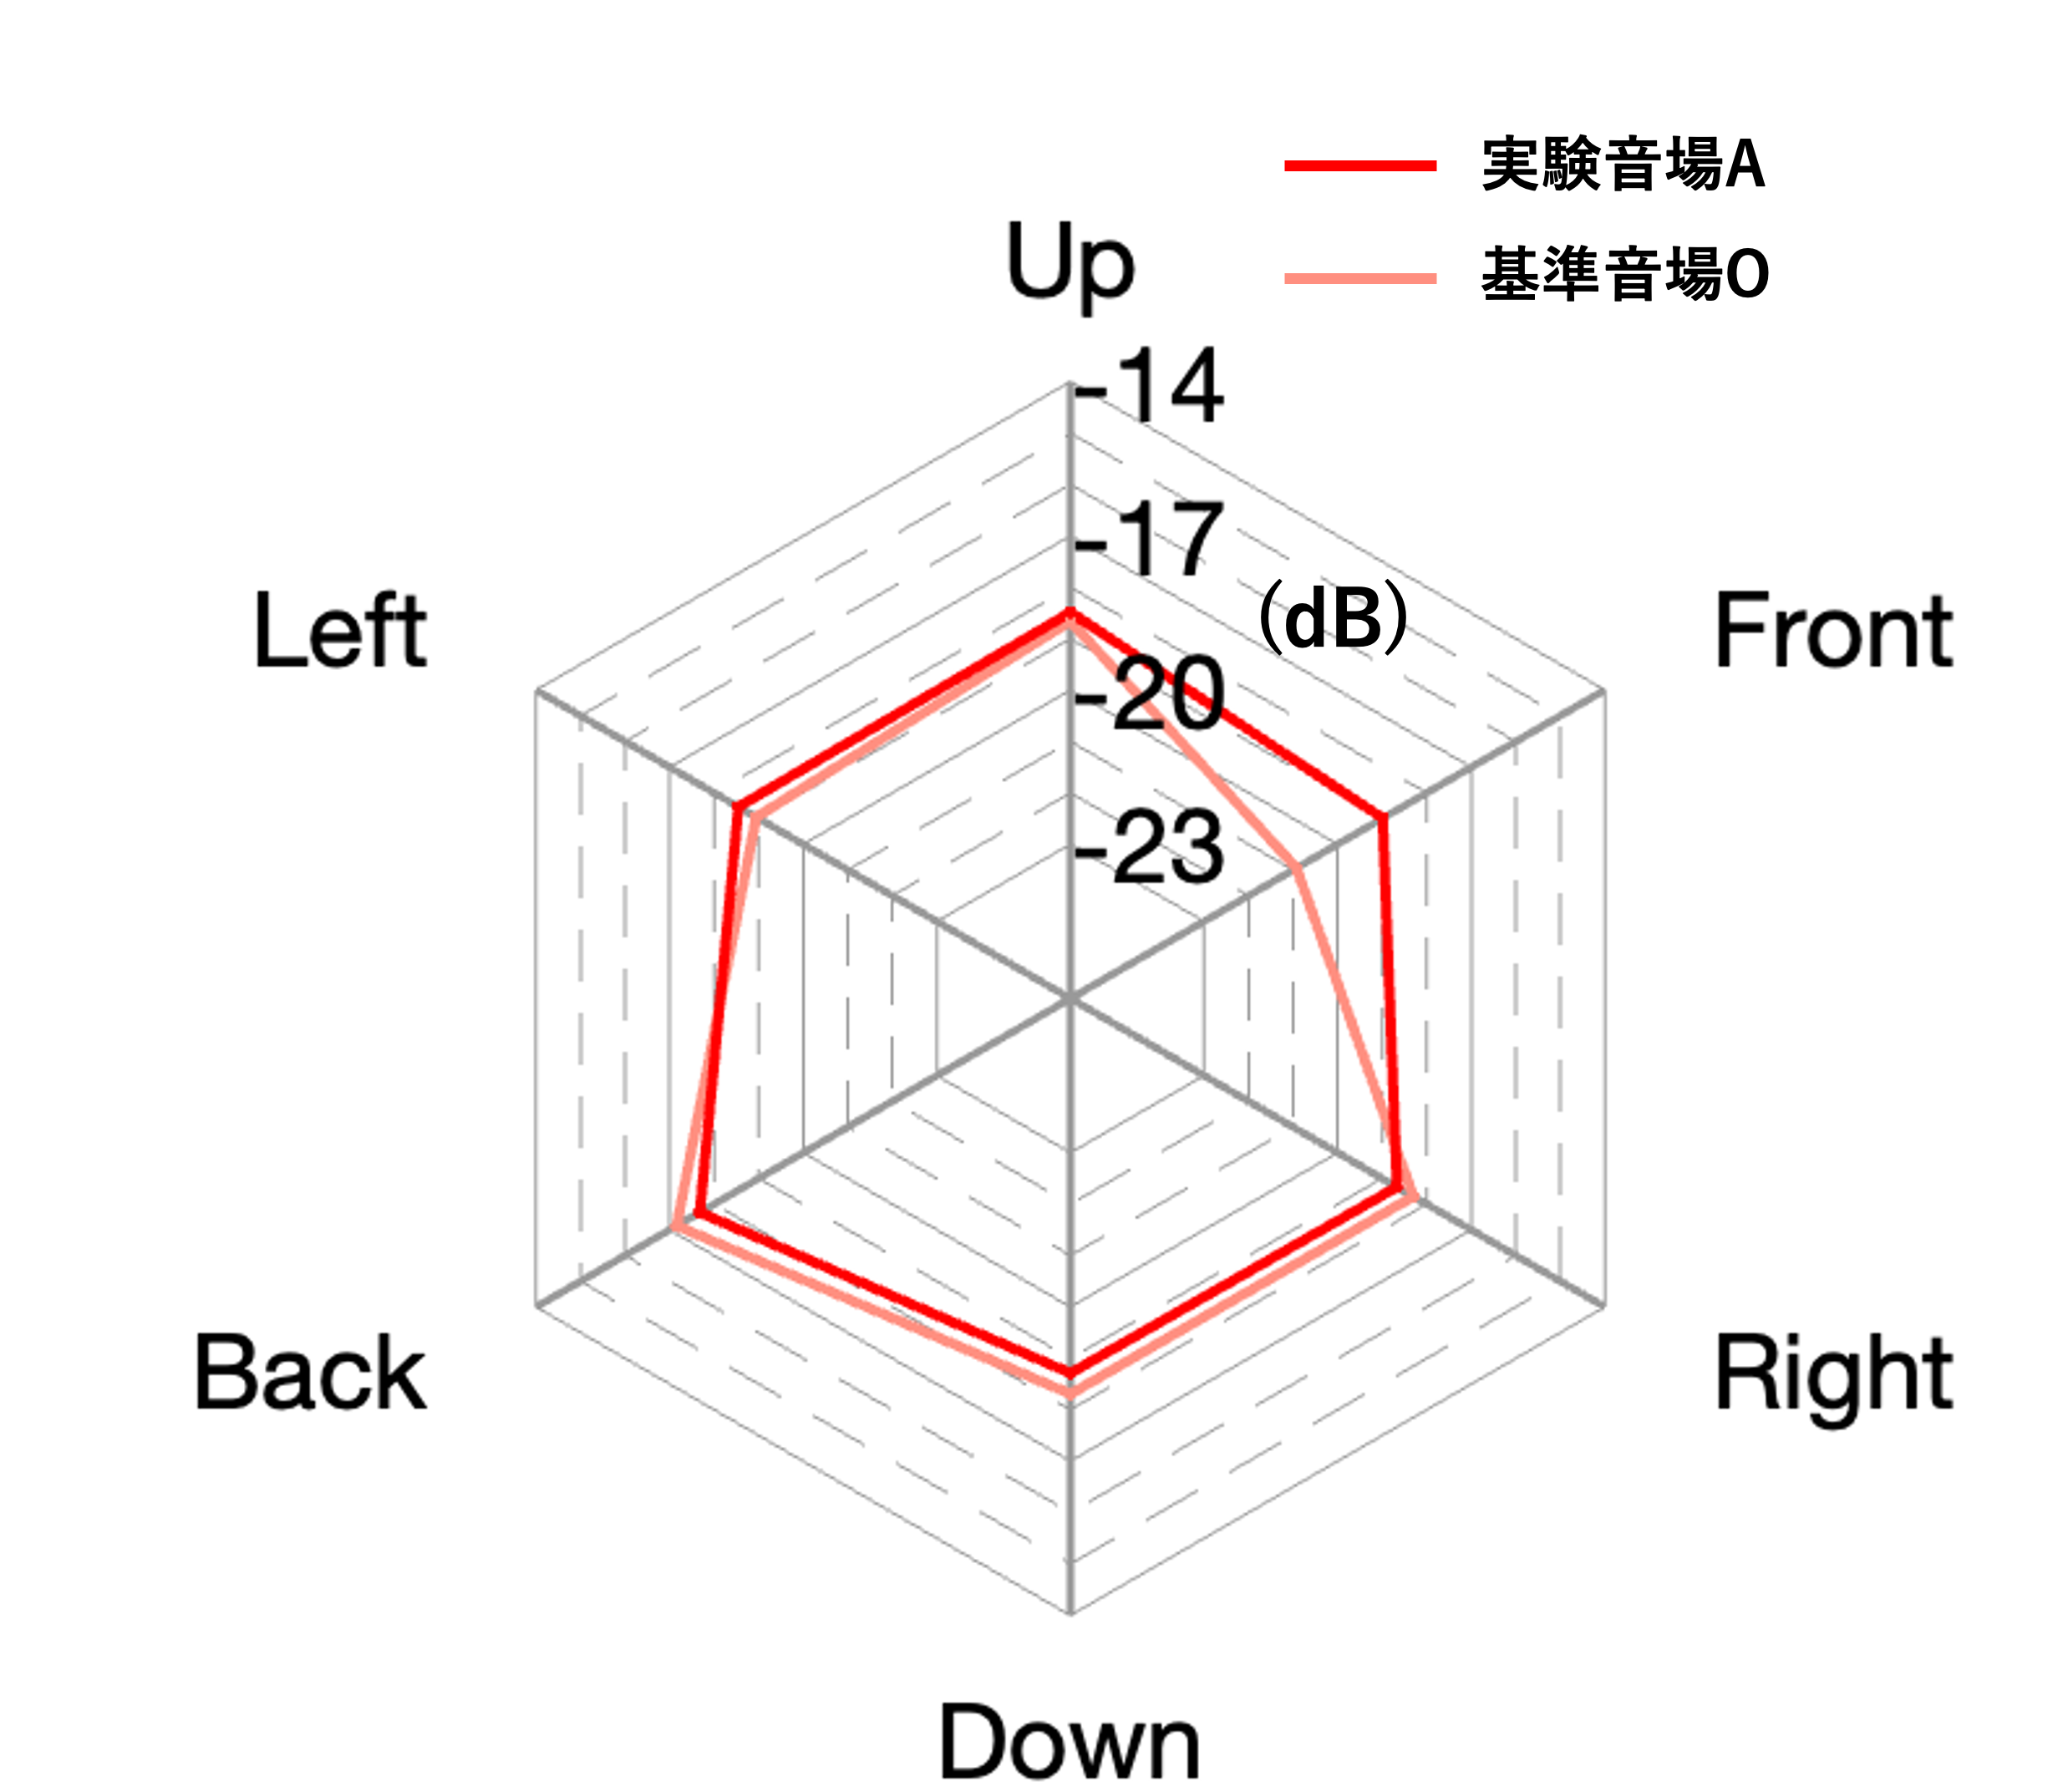
\includegraphics[width=1\linewidth]{images/experimentField/withLegend/expAEarly.png}
        \subcaption*{$\mathrm{ST_{Early,dir}}$\\前方強め}
    \end{minipage}%
    \begin{minipage}[b]{.5\linewidth}
        \centering
        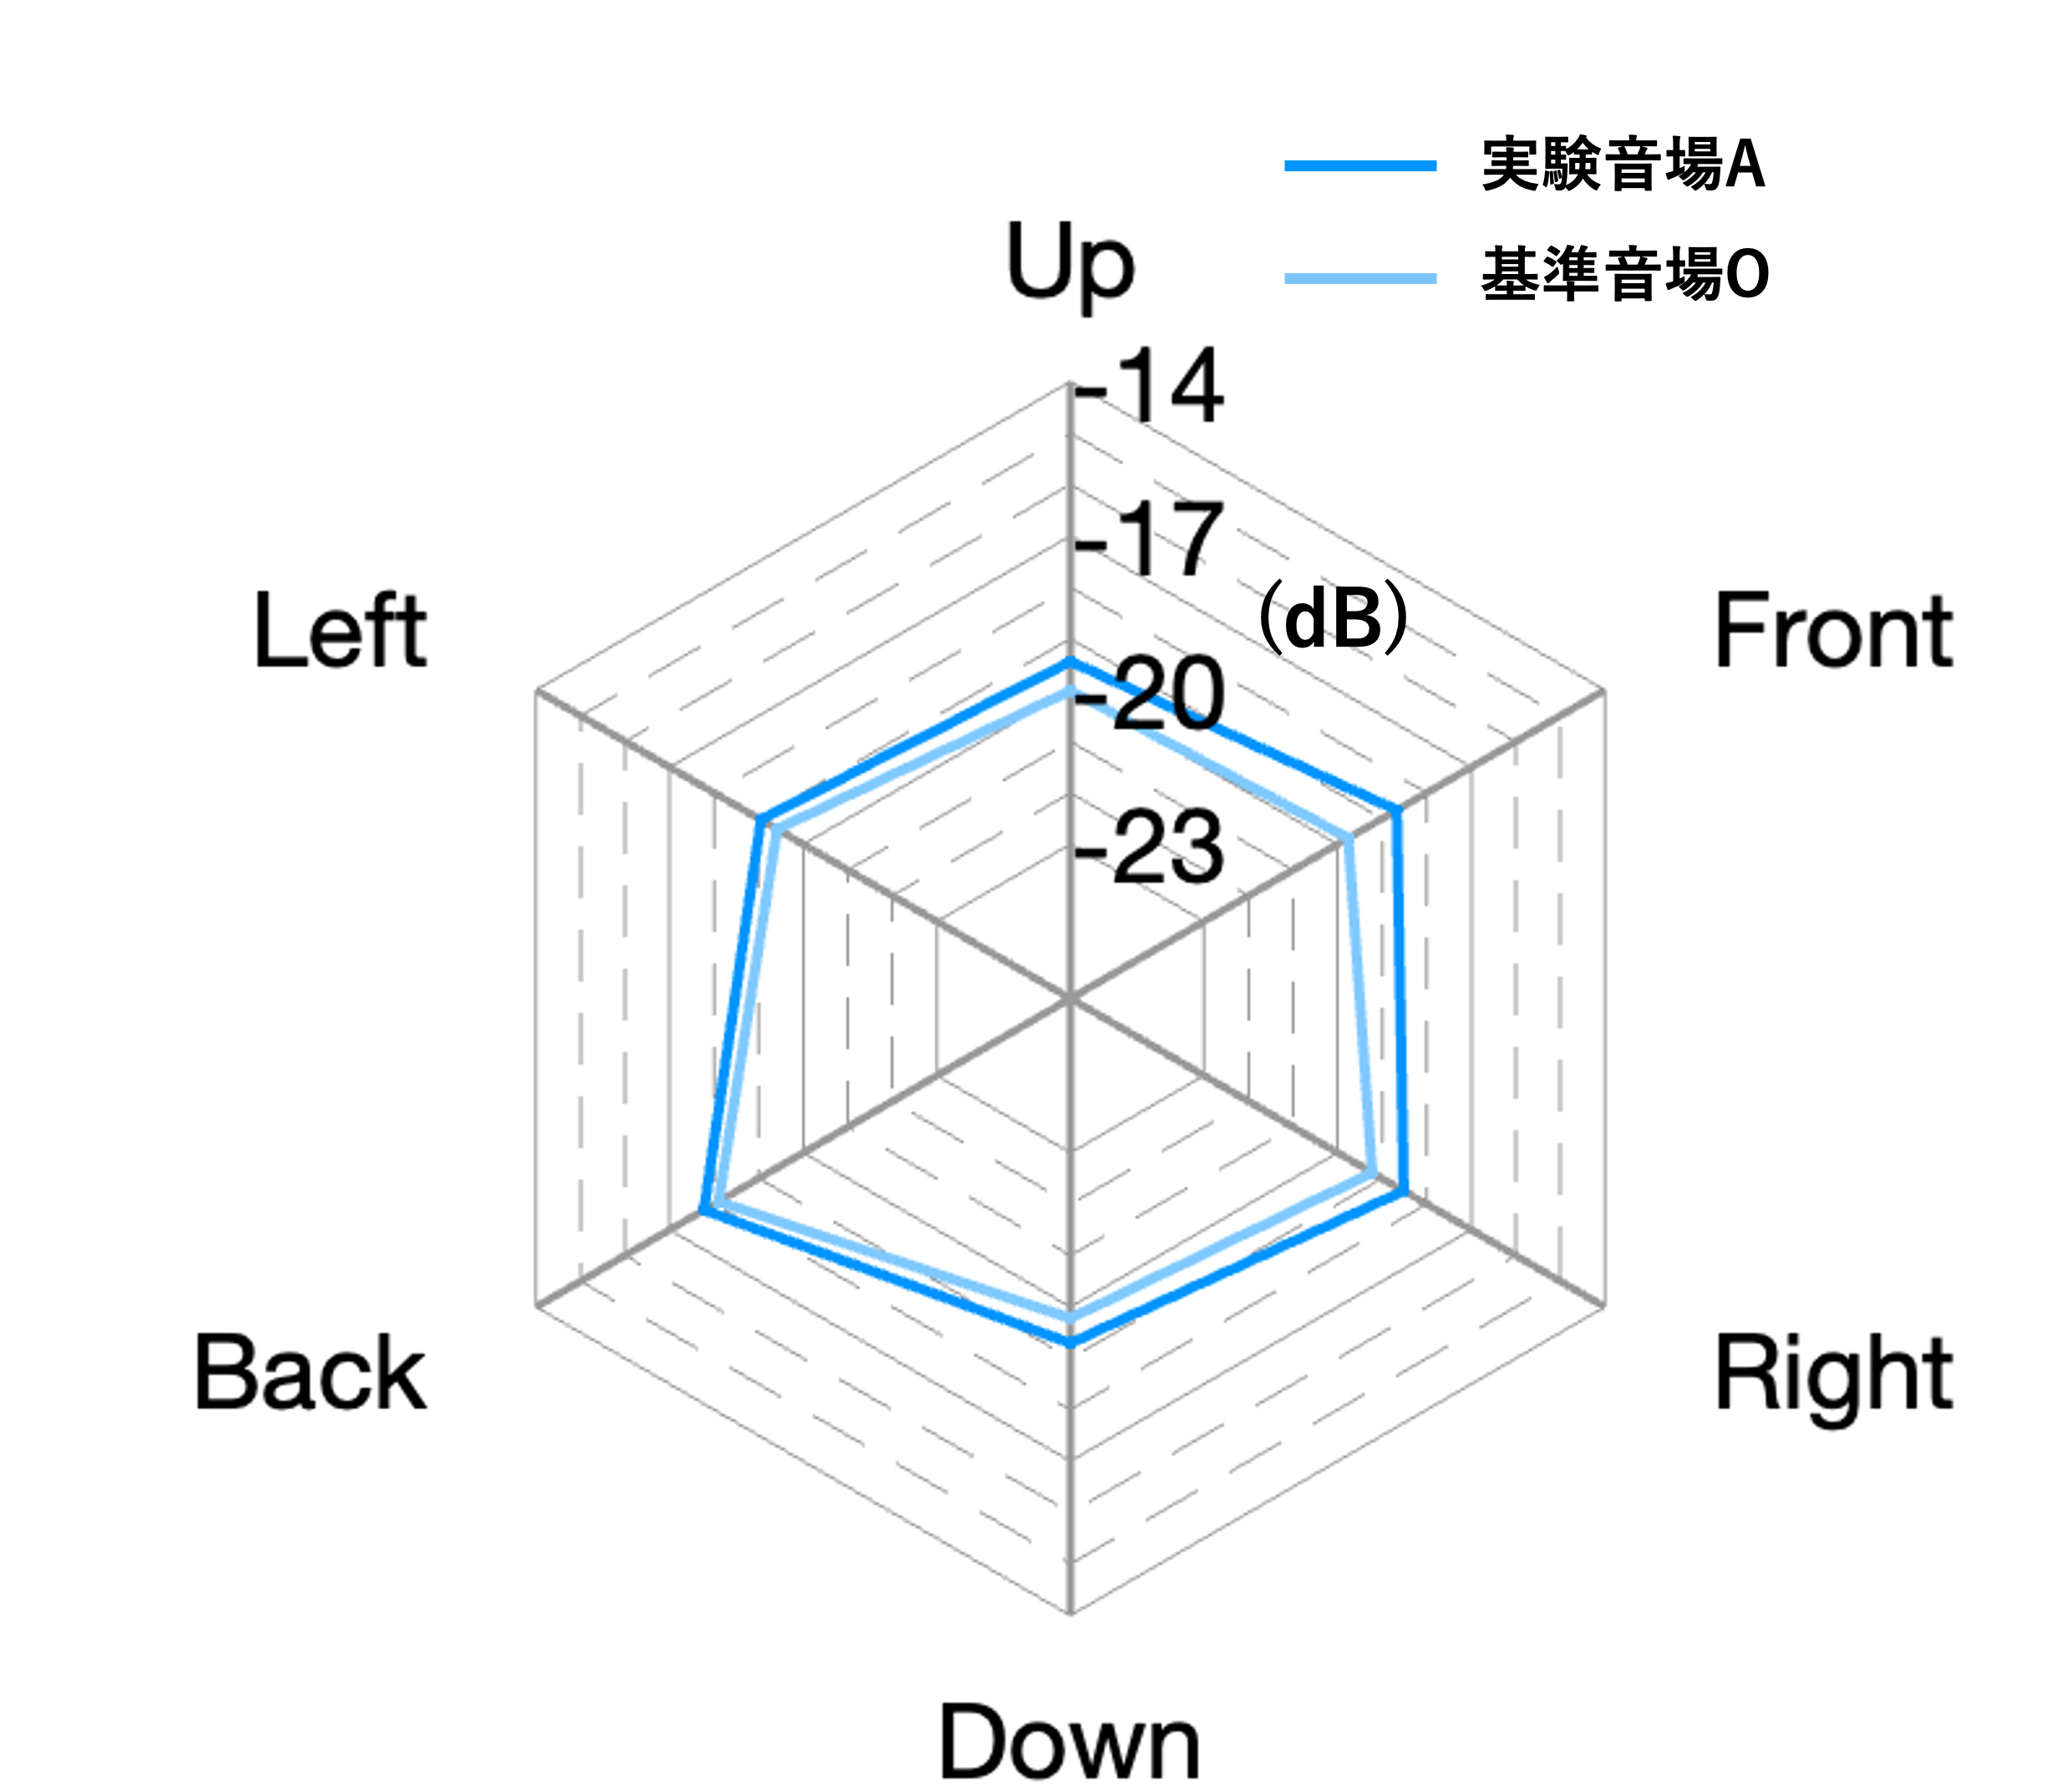
\includegraphics[width=1\linewidth]{images/experimentField/withLegend/expALate.png}
        \subcaption*{$\mathrm{ST_{Late,dir}}$\\基準音場と同じ}
    \end{minipage}
    \caption{音場Aの方向別ST}
    \label{fig:音場Aの方向別ST}
  \end{figure}

  \begin{figure}[H]
    \begin{minipage}[b]{.5\linewidth}
      \centering
      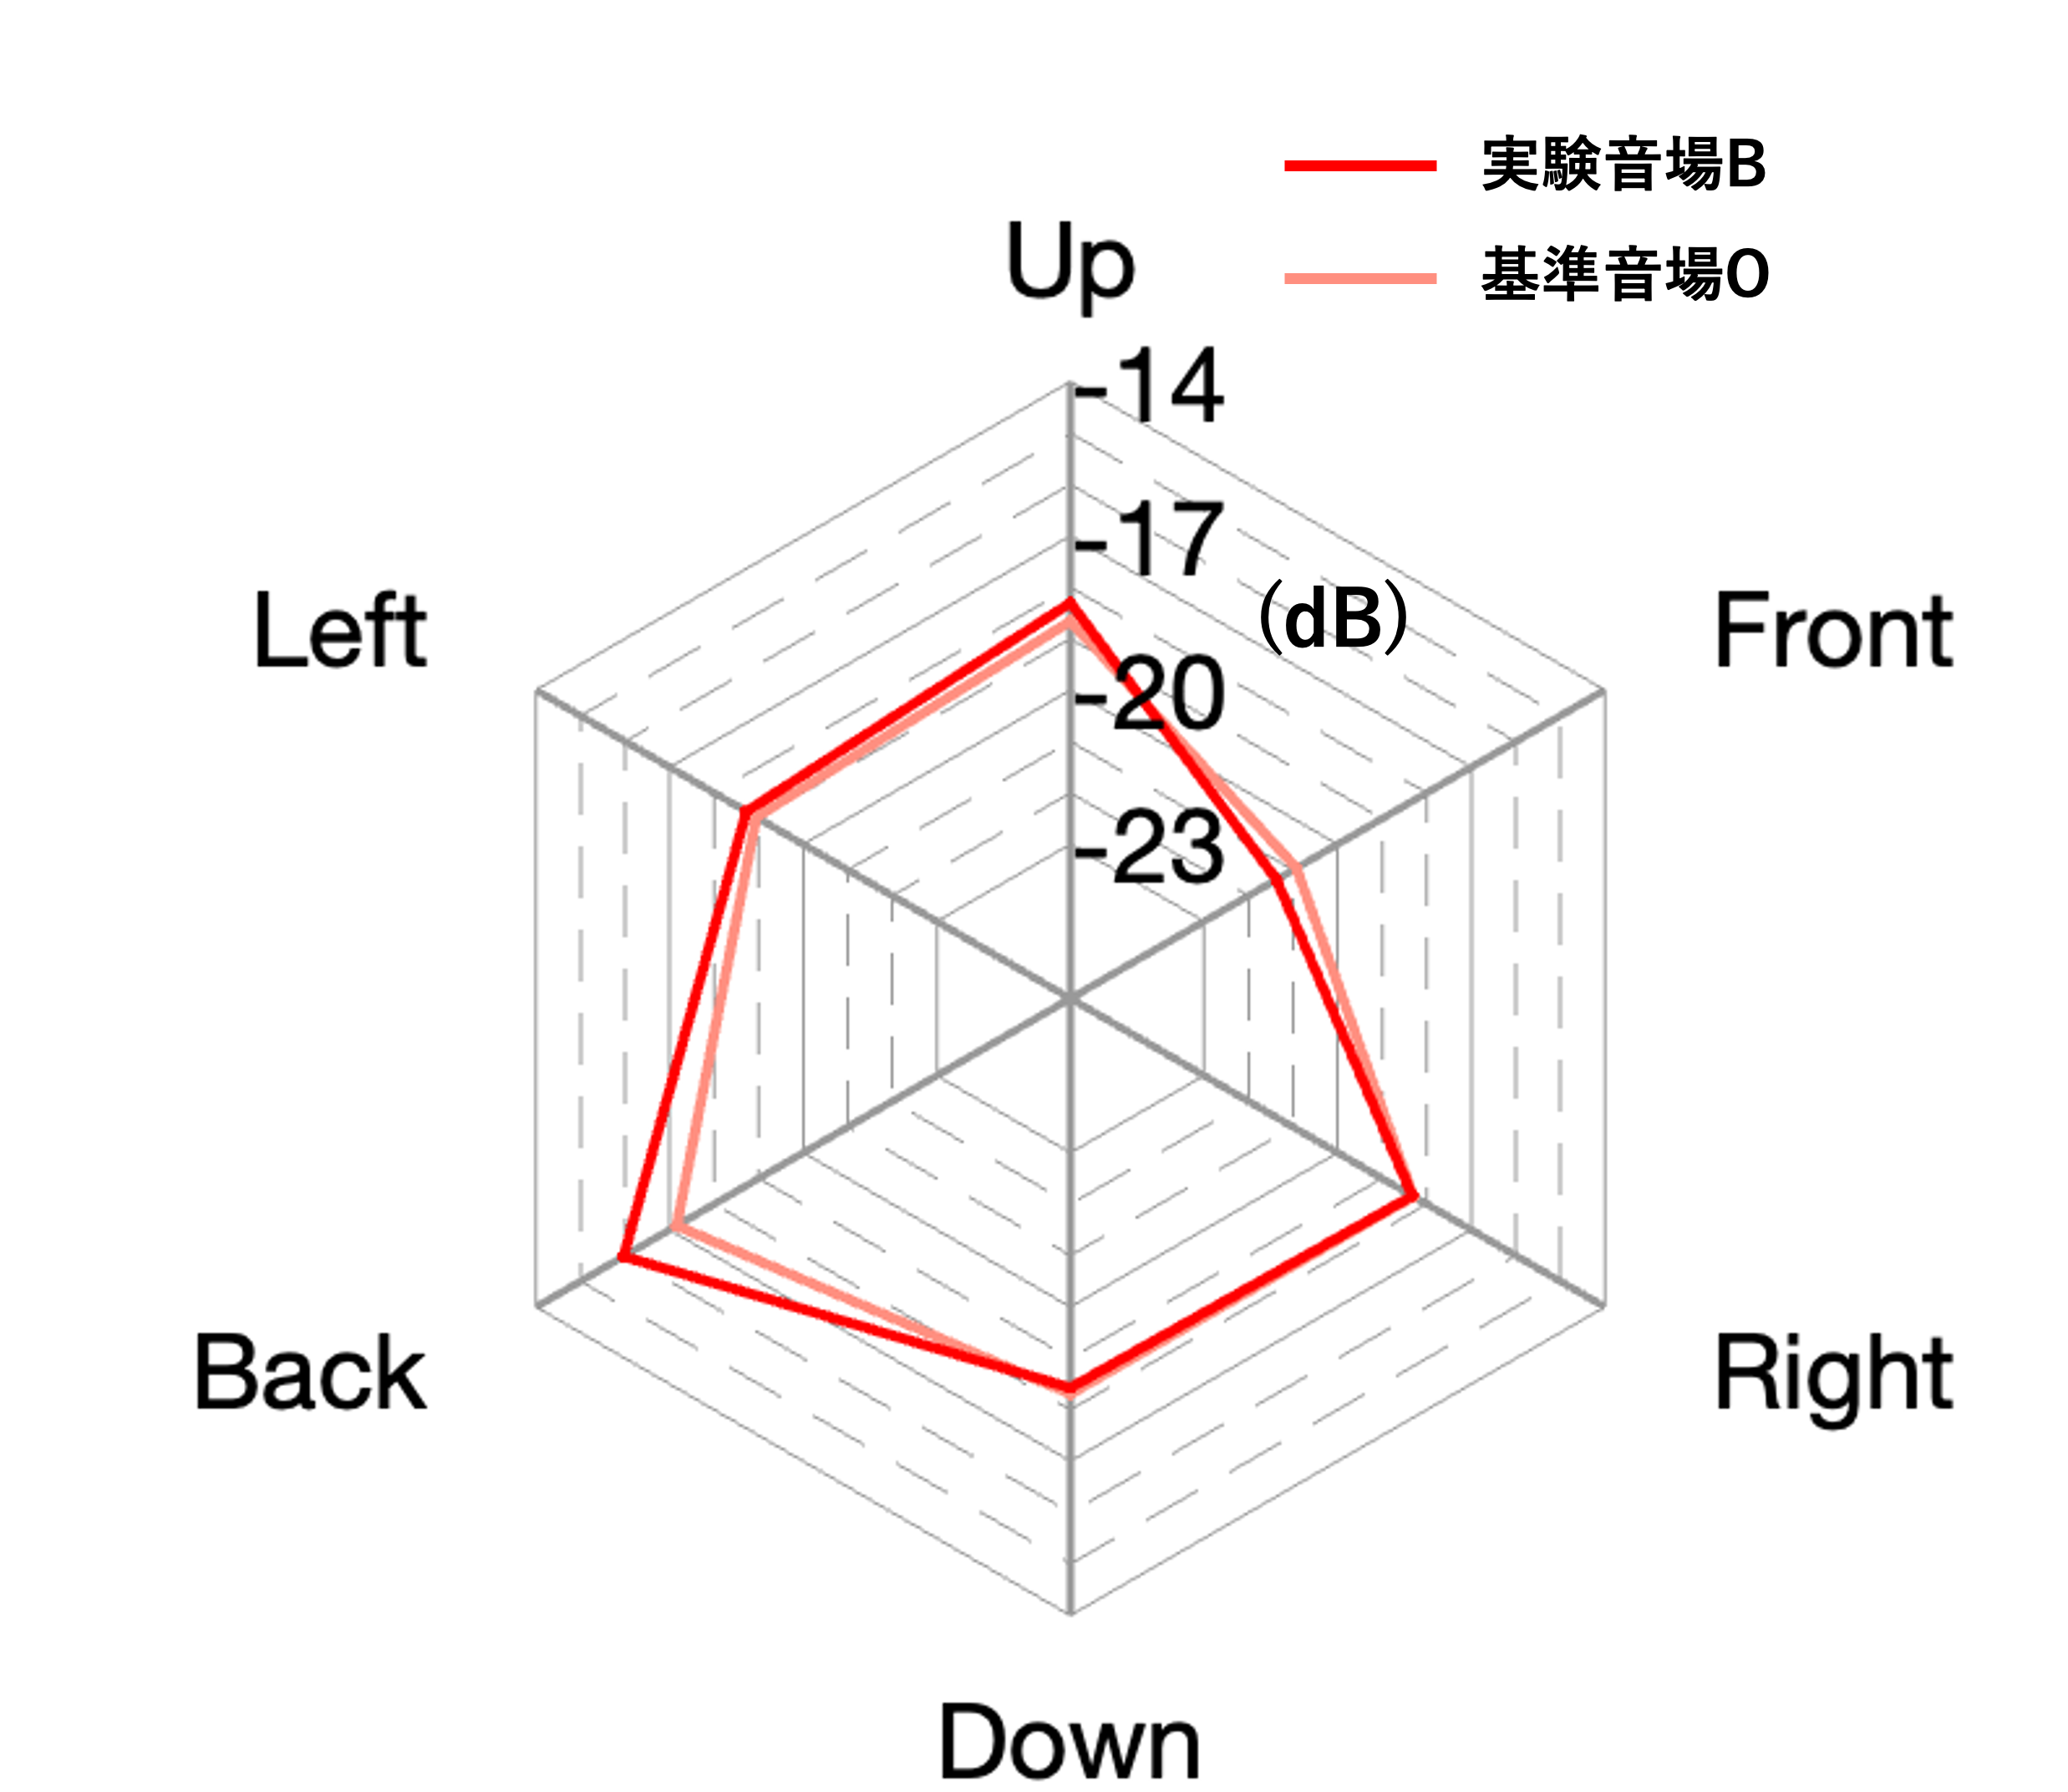
\includegraphics[width=1\linewidth]{images/experimentField/withLegend/expBEarly.png}
      \subcaption*{$\mathrm{ST_{Early,dir}}$\\後方強め}
    \end{minipage}%
    \begin{minipage}[b]{.5\linewidth}
        \centering
        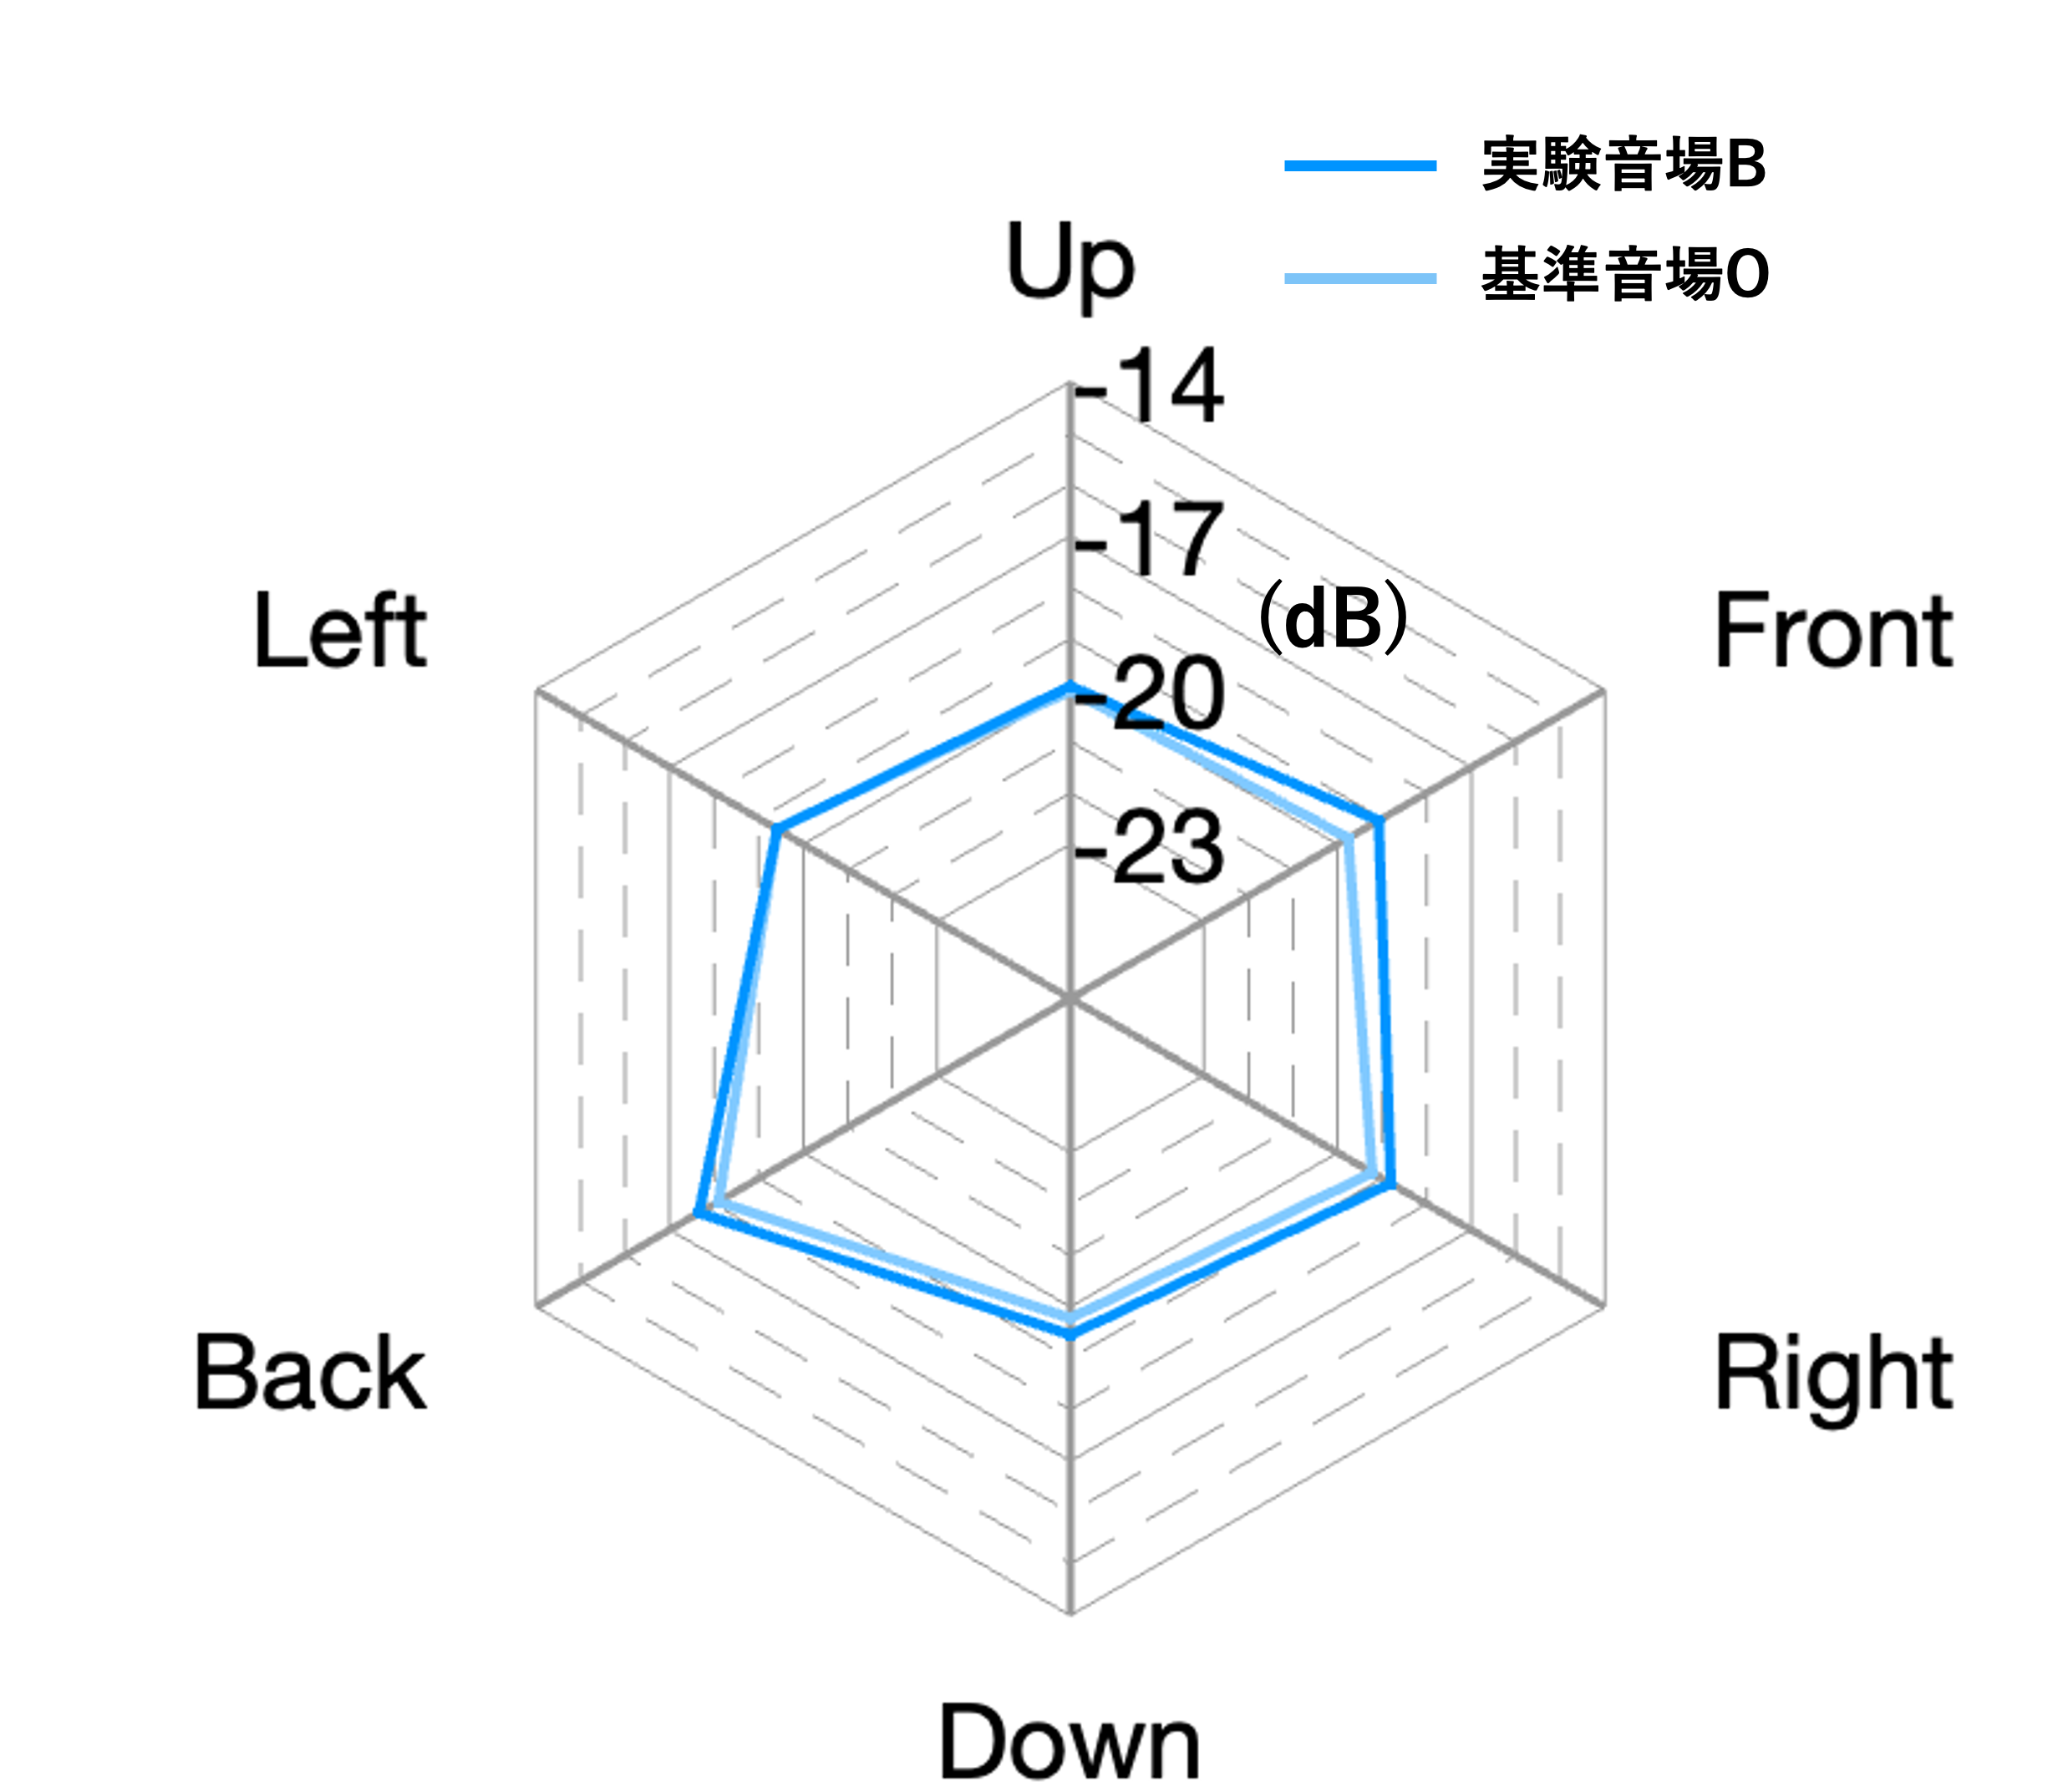
\includegraphics[width=1\linewidth]{images/experimentField/withLegend/expBLate.png}
        \subcaption*{$\mathrm{ST_{Late,dir}}$\\基準音場と同じ}
    \end{minipage}
    \caption{音場Bの方向別ST}
    \label{fig:音場Bの方向別ST}
  \end{figure}

  \newpage

  \begin{figure}[H]
    \begin{minipage}[b]{.5\linewidth}
      \centering
      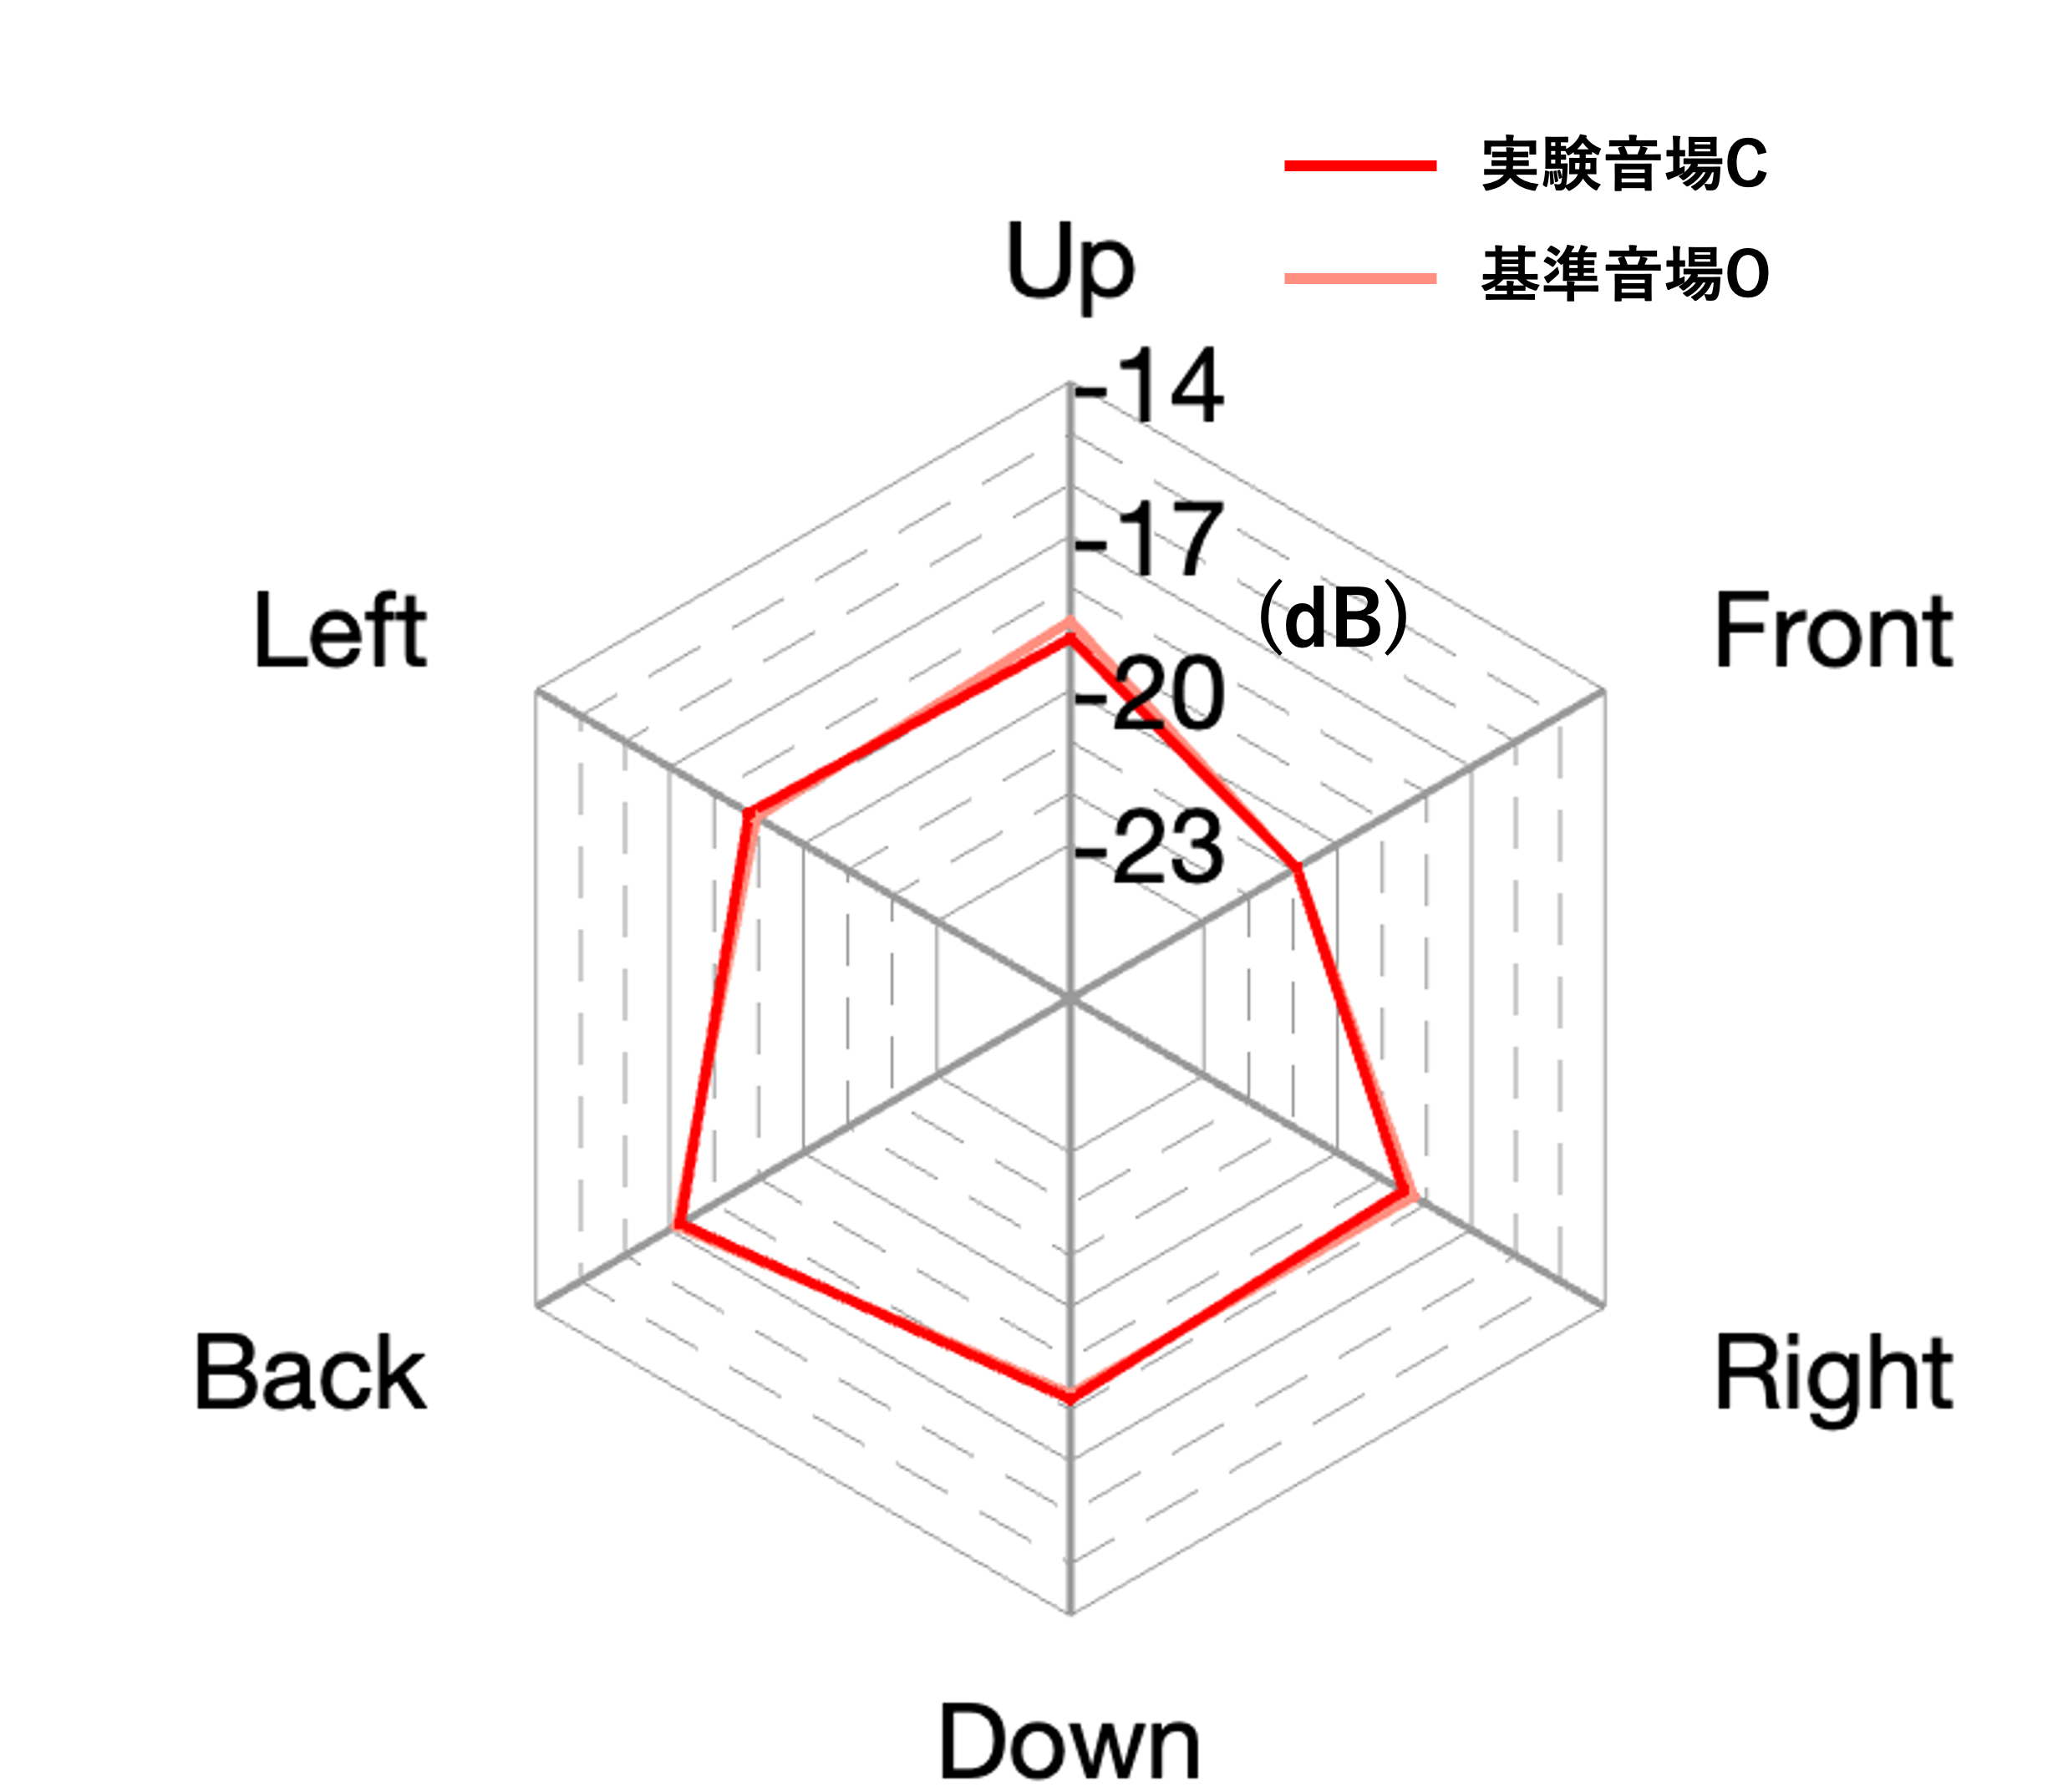
\includegraphics[width=1\linewidth]{images/experimentField/withLegend/expCEarly.png}
      \subcaption*{$\mathrm{ST_{Early,dir}}$\\基準音場と同じ}
    \end{minipage}%
    \begin{minipage}[b]{.5\linewidth}
        \centering
        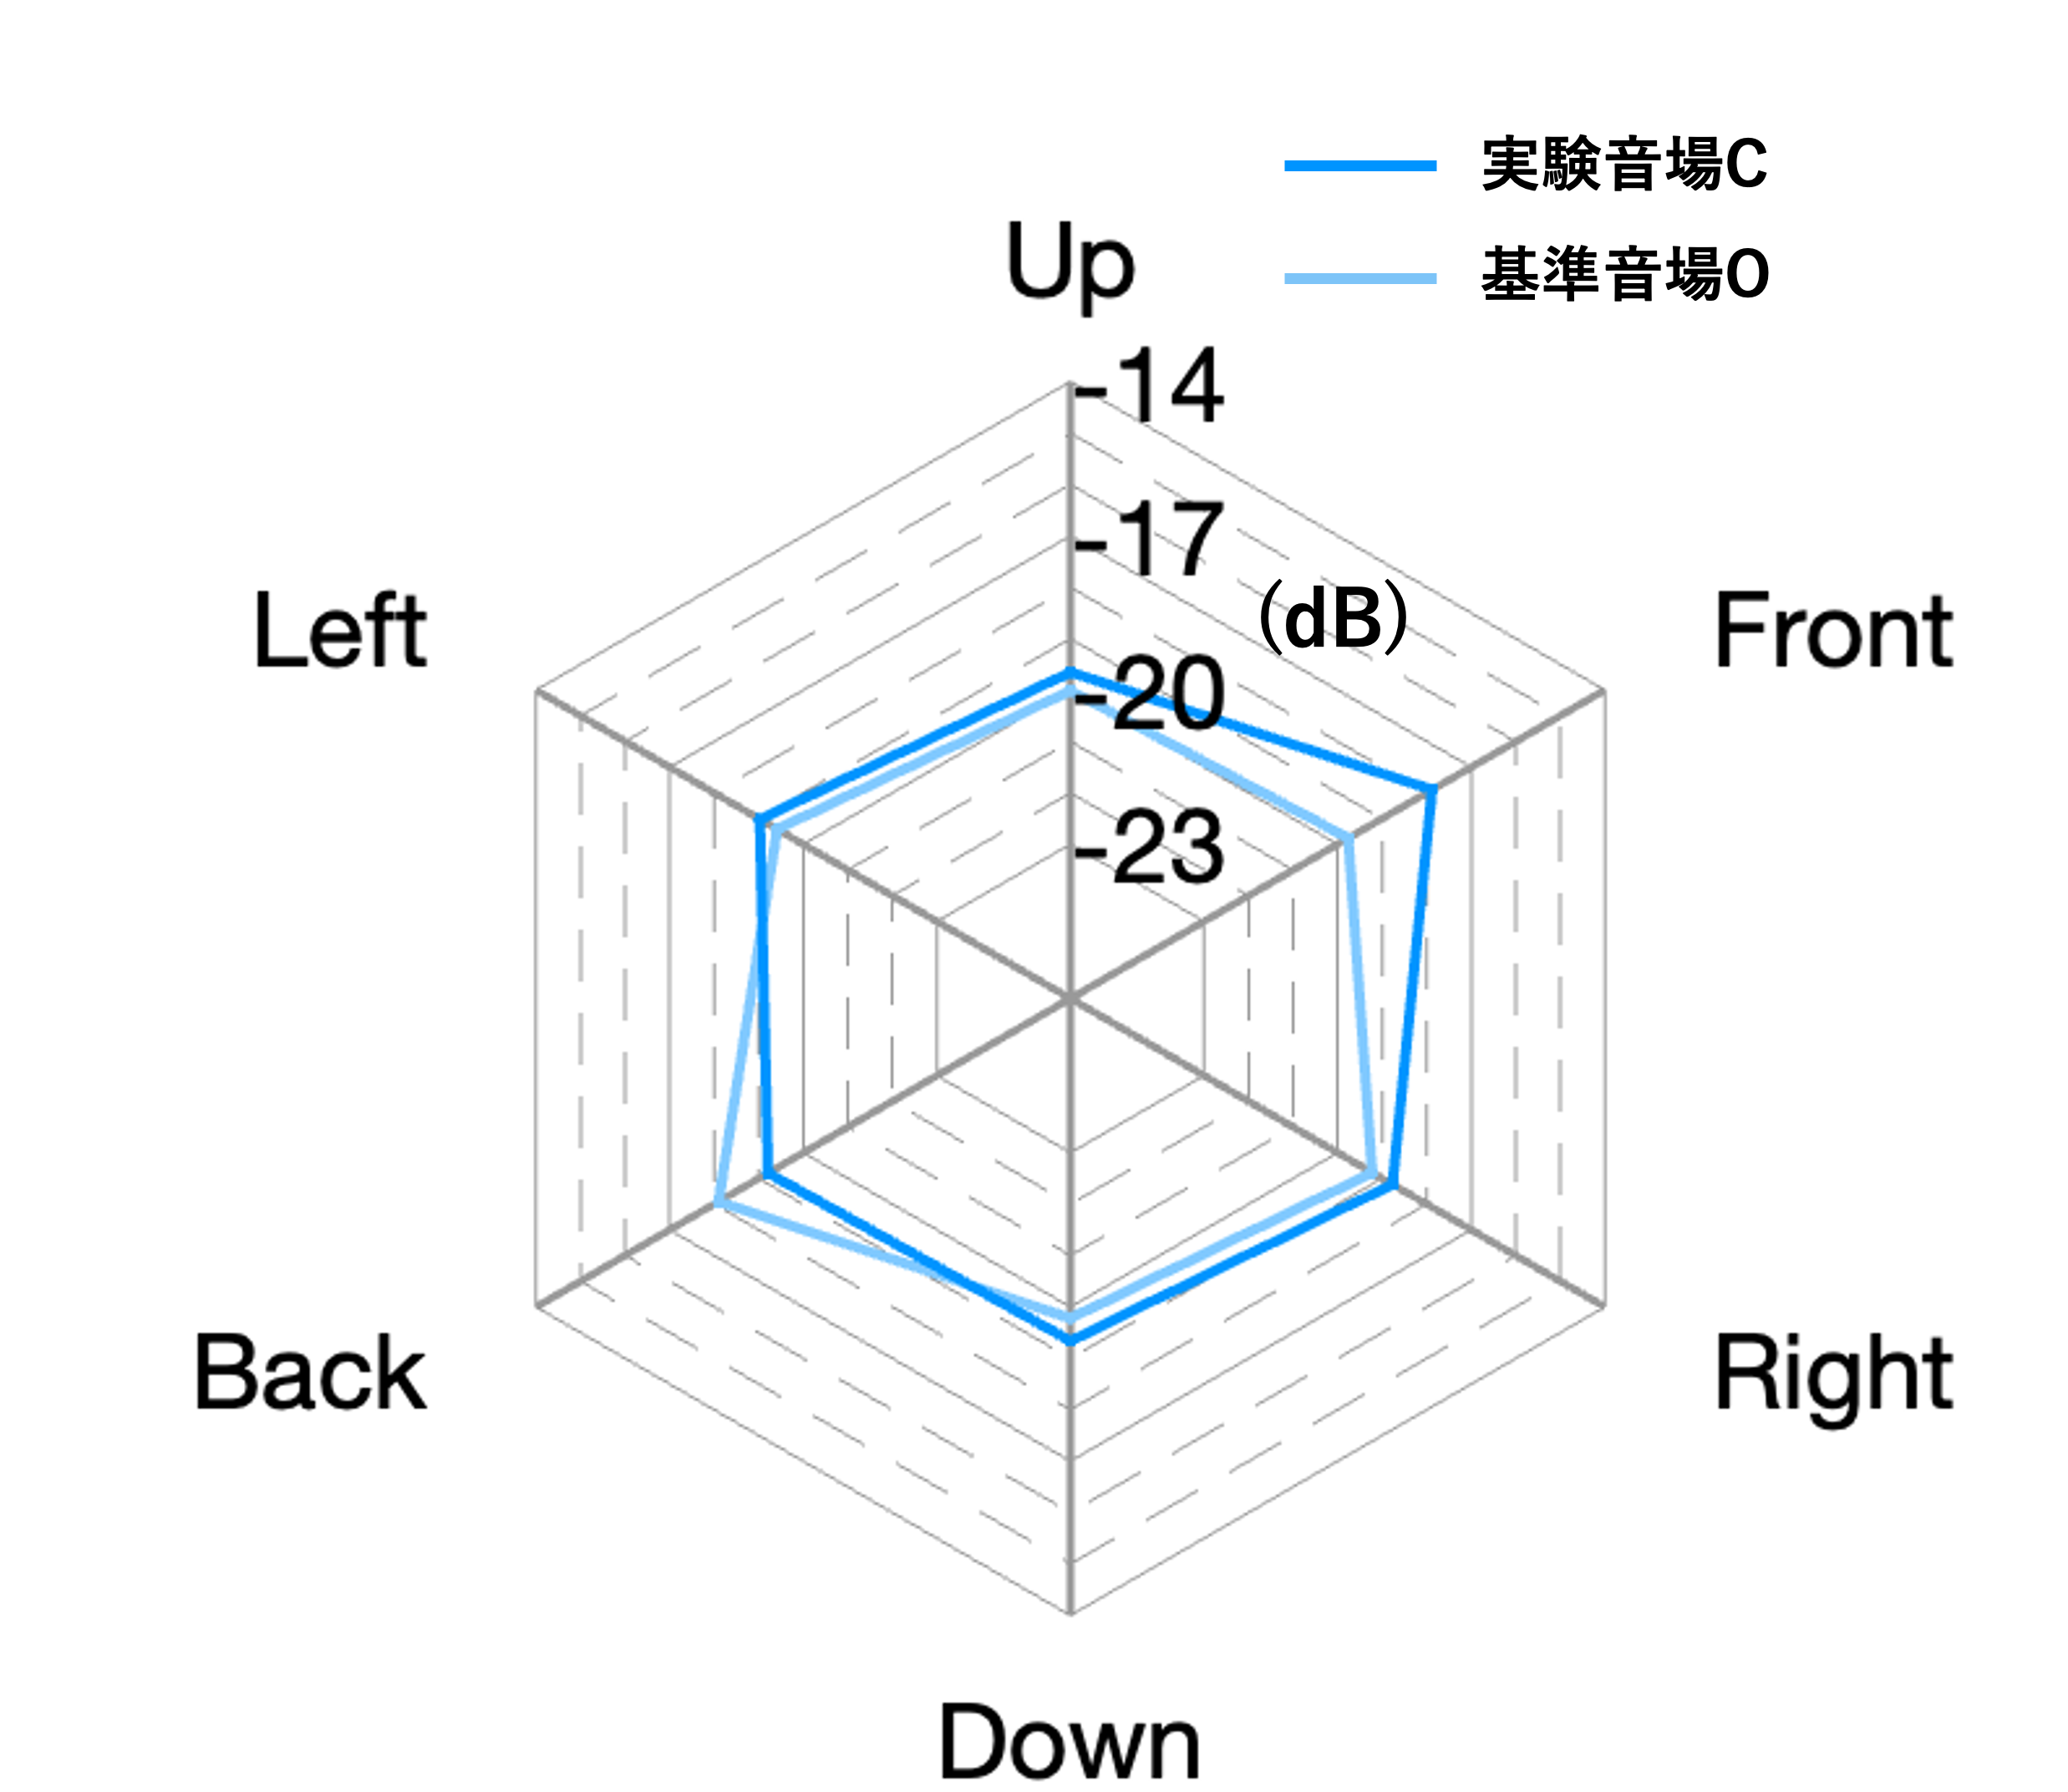
\includegraphics[width=1\linewidth]{images/experimentField/withLegend/expCLate.png}
        \subcaption*{$\mathrm{ST_{Late,dir}}$\\前方強め}
    \end{minipage}
    \caption{音場Cの方向別ST}
    \label{fig:音場Cの方向別ST}
  \end{figure}

  \begin{figure}[H]
    \begin{minipage}[b]{.5\linewidth}
        \centering
        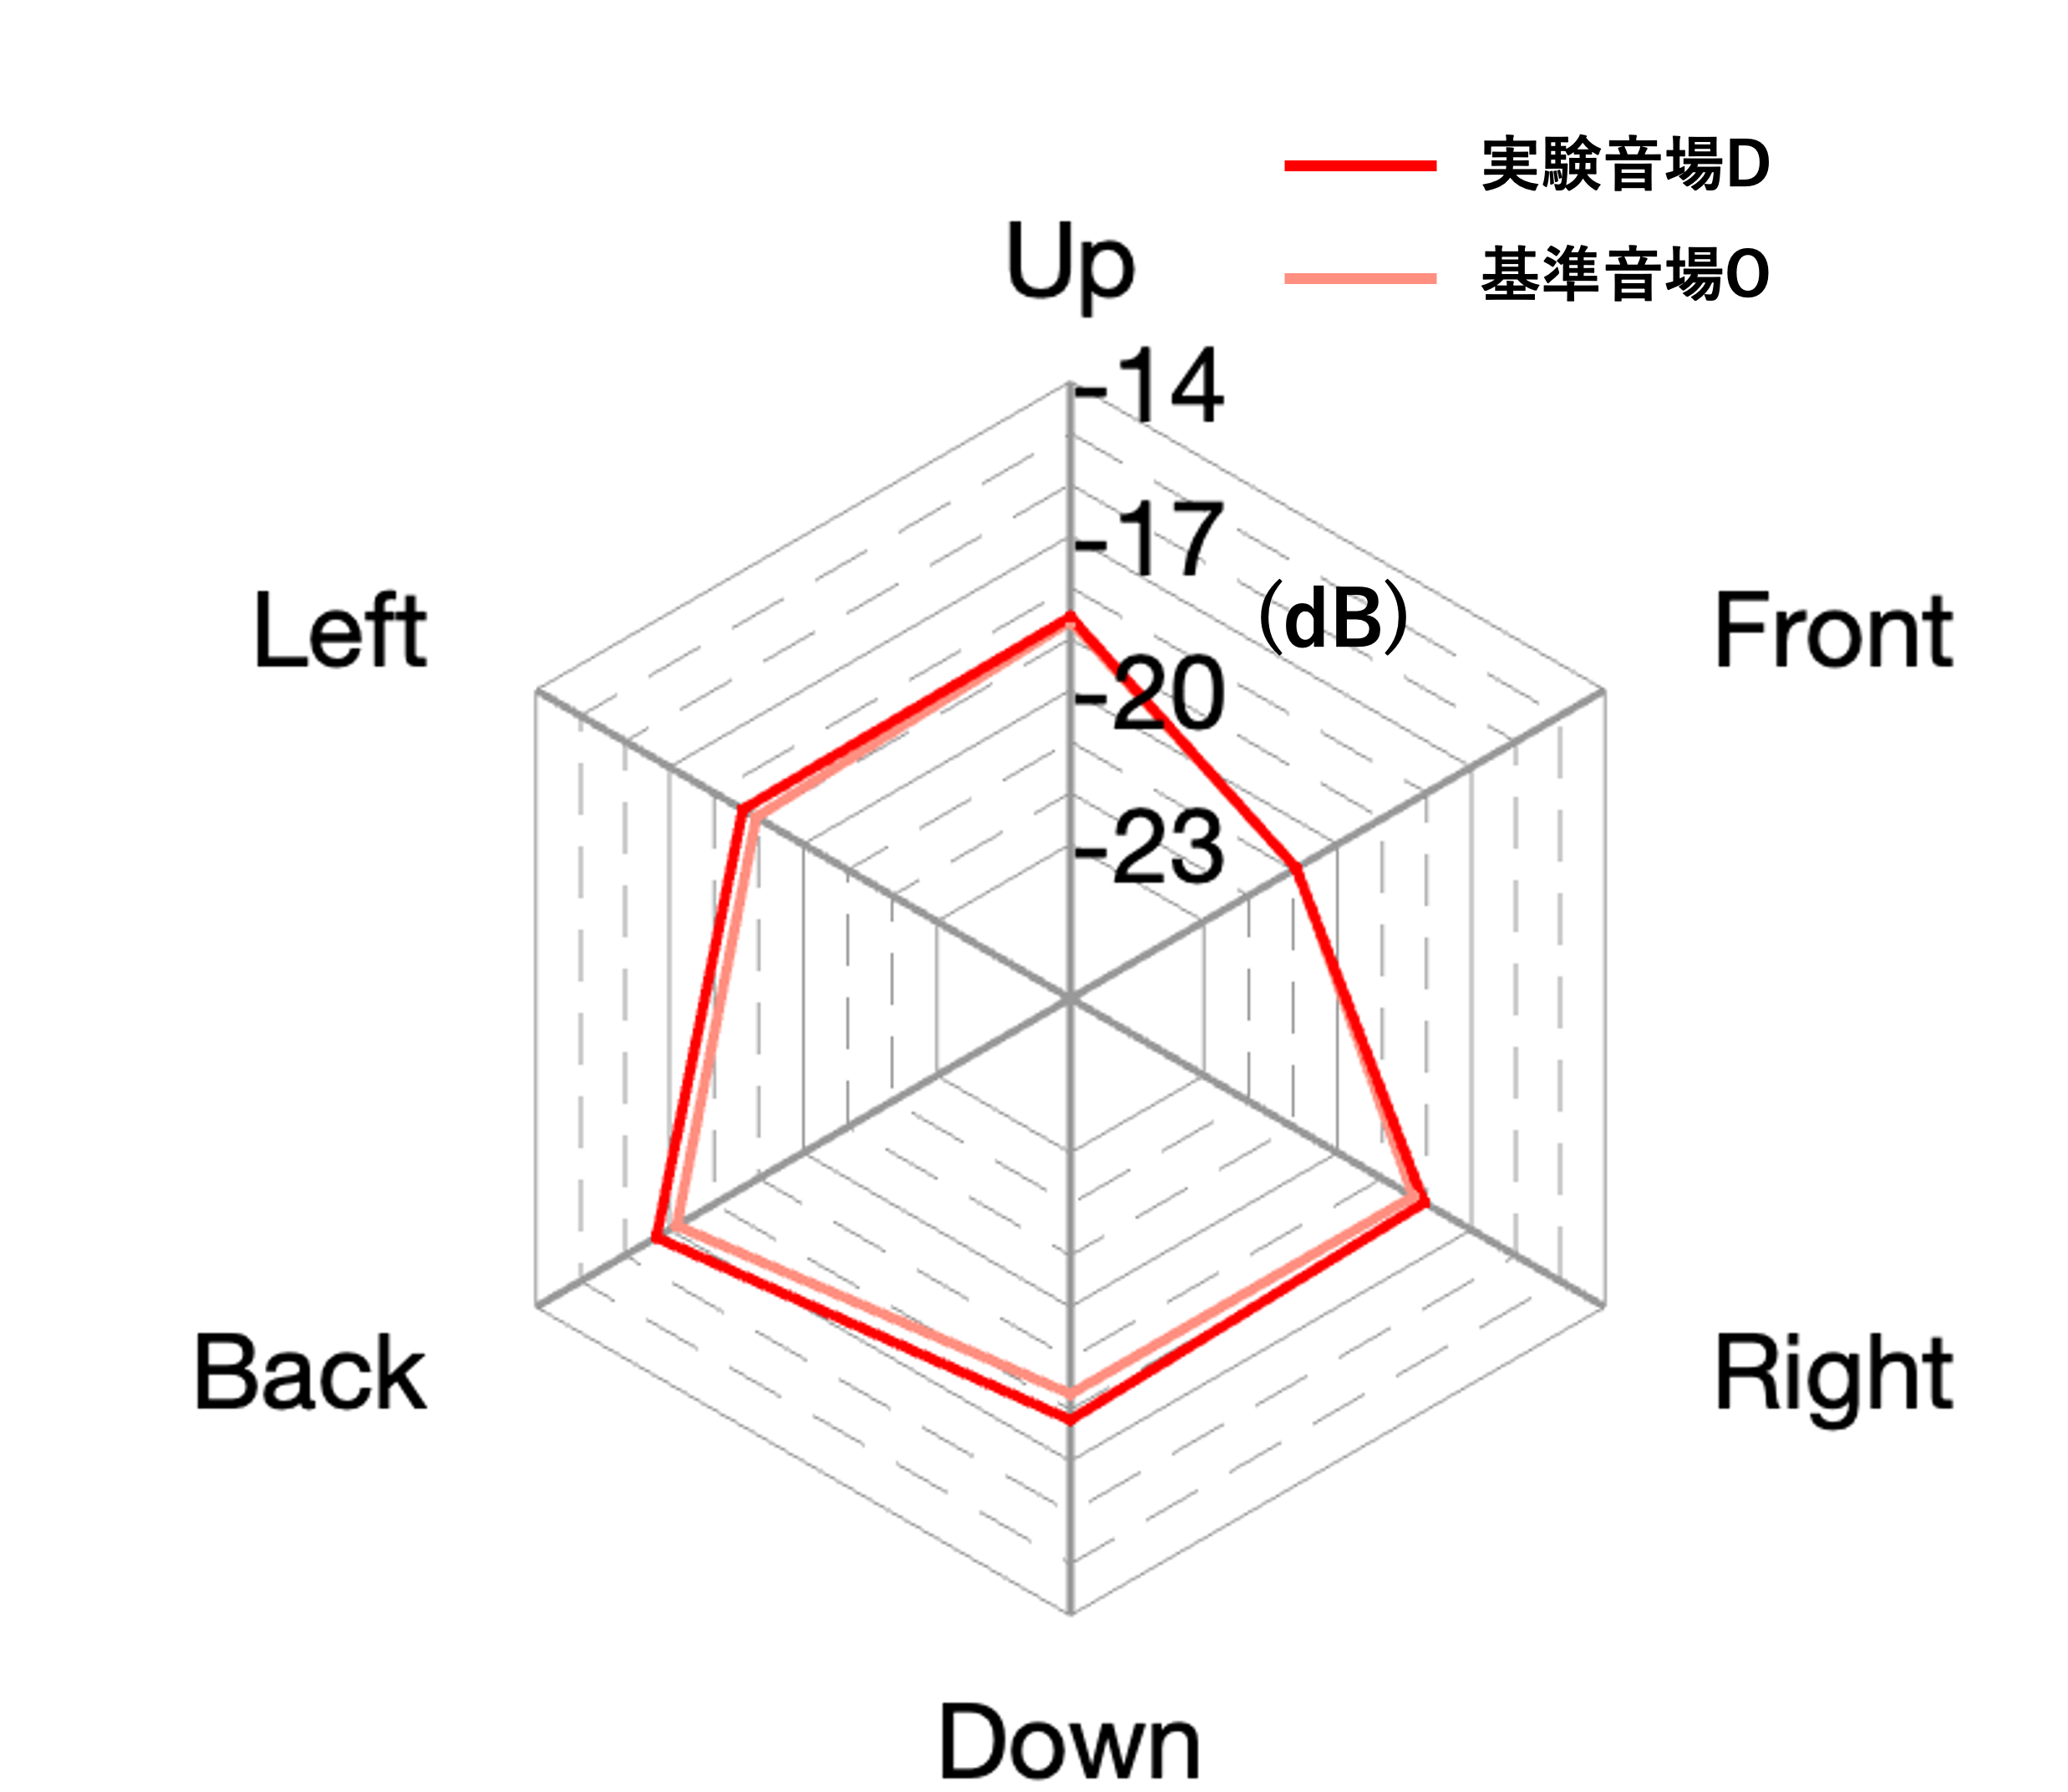
\includegraphics[width=1\linewidth]{images/experimentField/withLegend/expDEarly.png}
        \subcaption*{$\mathrm{ST_{Early,dir}}$\\基準音場と同じ}
    \end{minipage}%
    \begin{minipage}[b]{.5\linewidth}
        \centering
        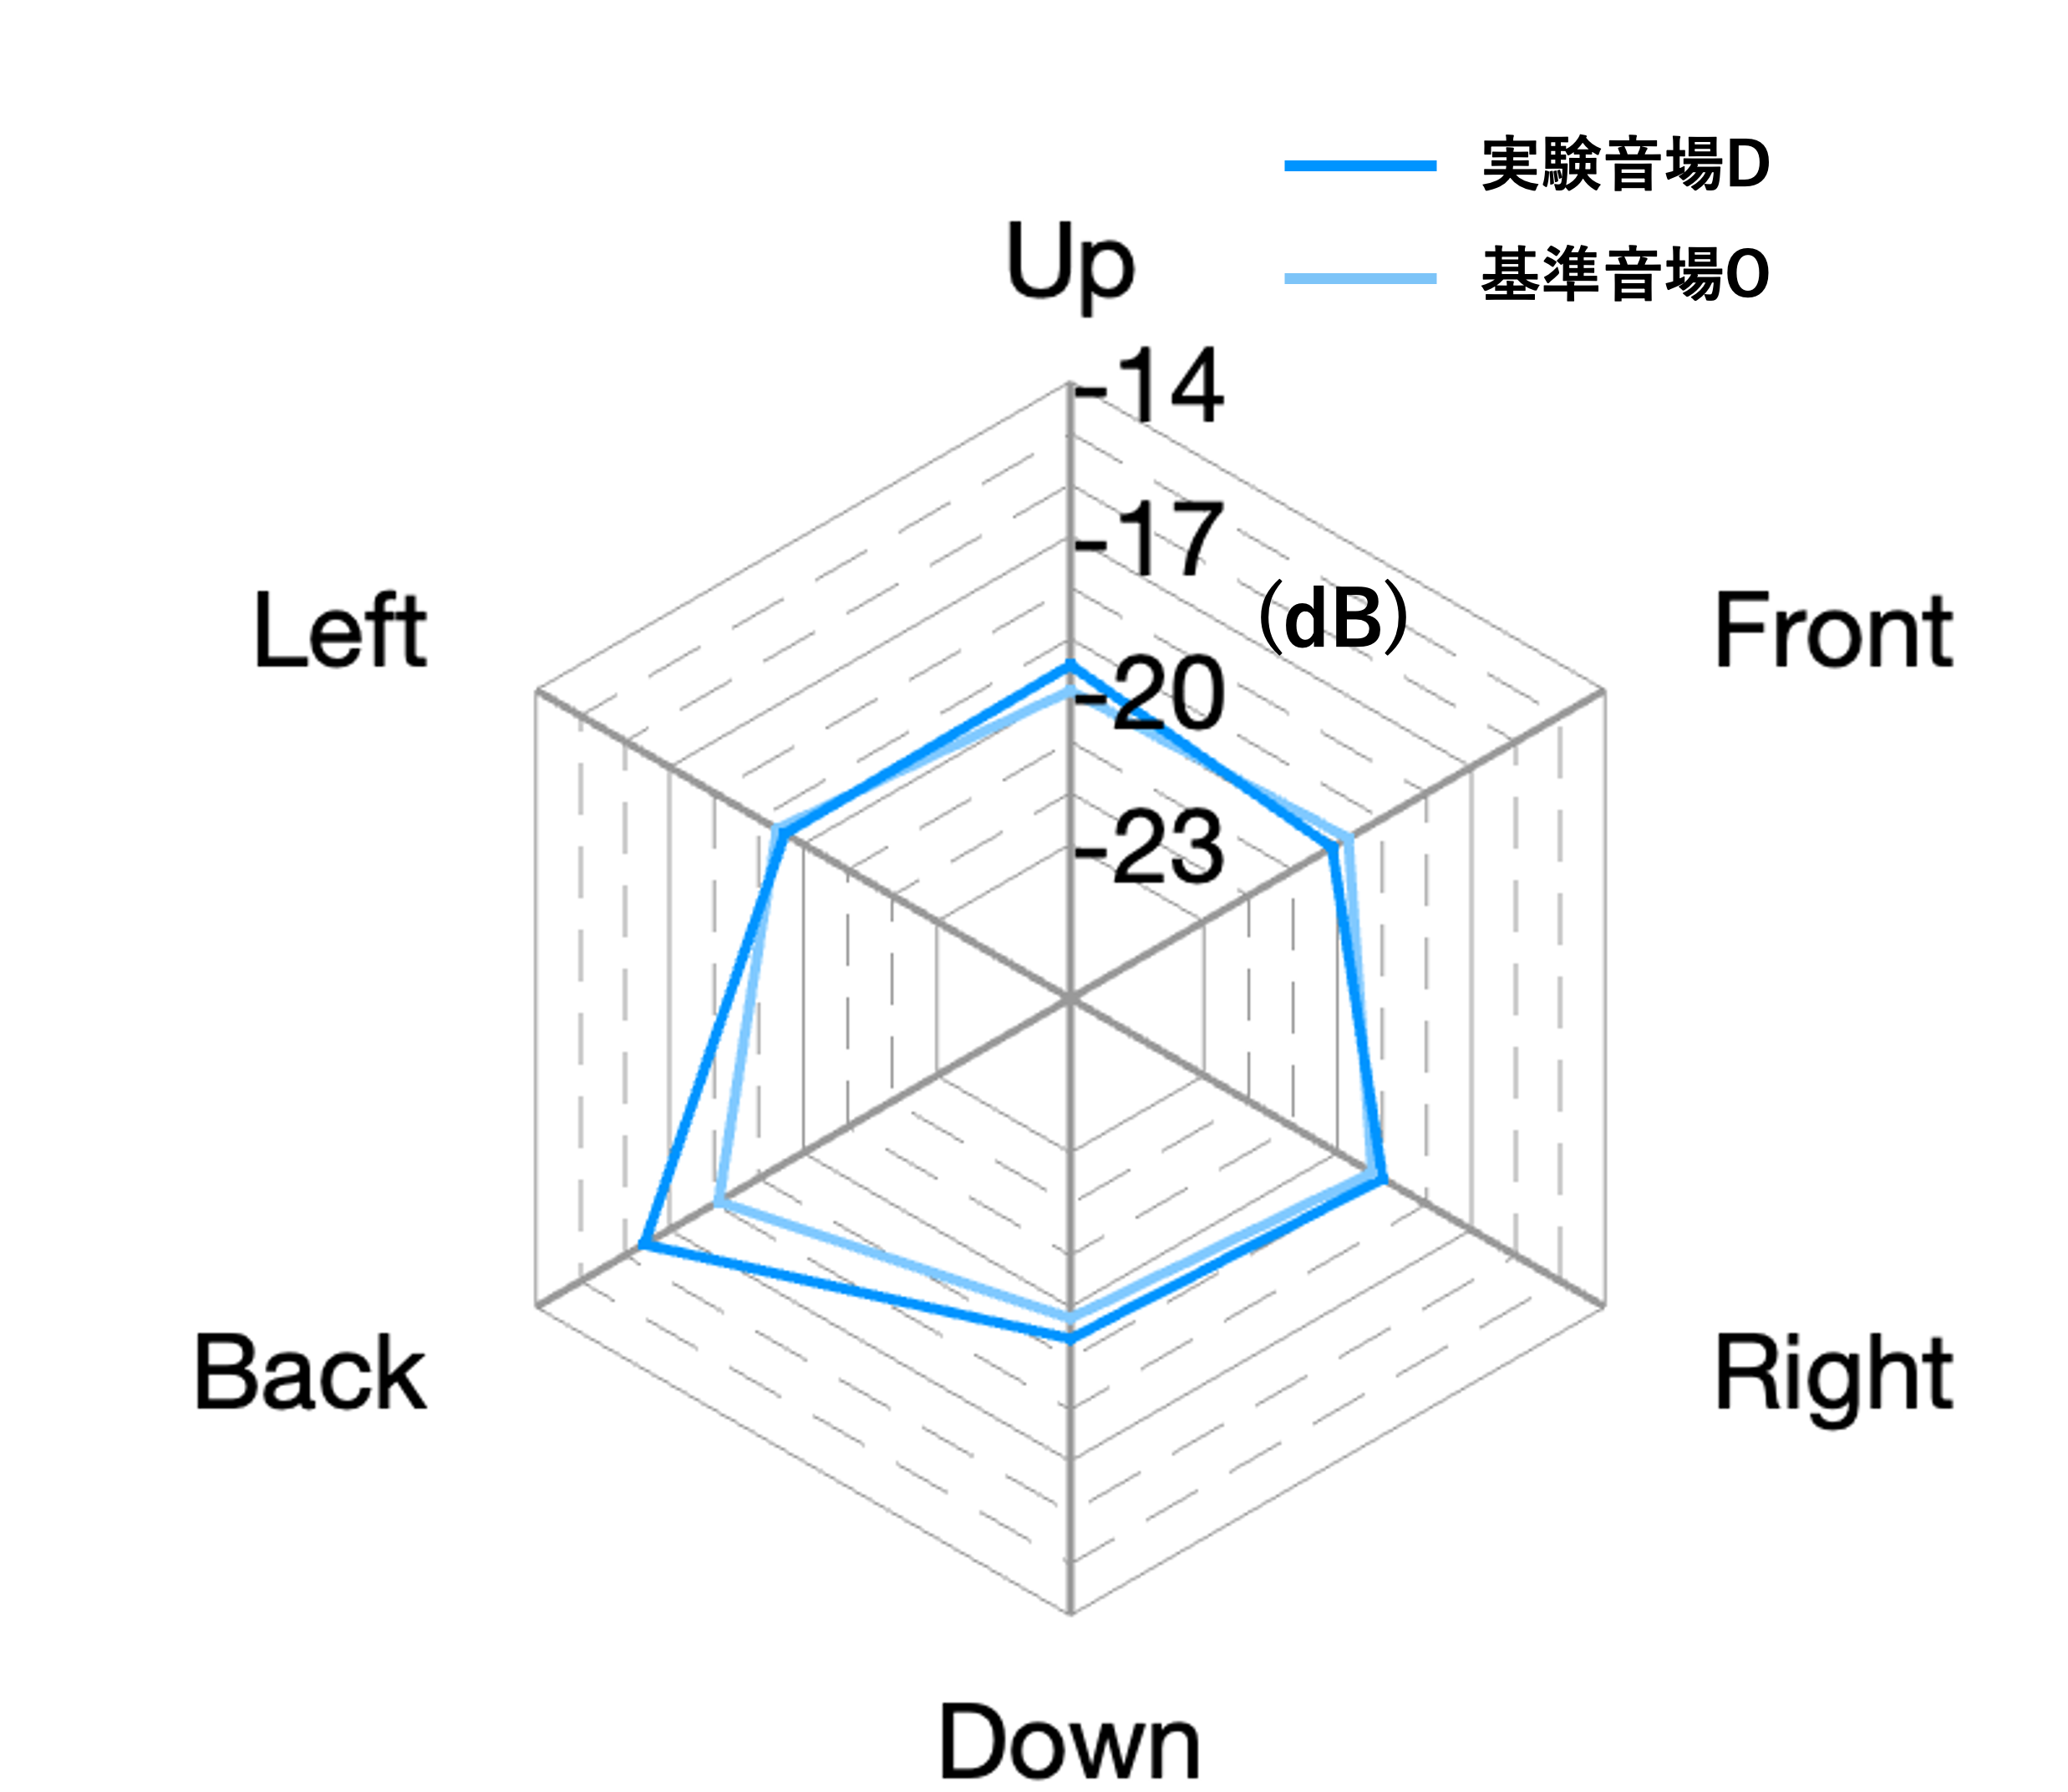
\includegraphics[width=1\linewidth]{images/experimentField/withLegend/expDLate.png}
        \subcaption*{$\mathrm{ST_{Late,dir}}$\\後方強め}
    \end{minipage}
    \caption{音場Dの方向別ST}
    \label{fig:音場Dの方向別ST}
  \end{figure}

%=====================================================================================




\clearpage

% 参考文献
% 参考文献の箇所にインプットしてください。

% 分割ファイル内でのみ,bibliographyを読み込みます。

\expandafter\ifx\csname ifdraft\endcsname\relax

  % bibliographyを展開する

  \bibliographystyle{junsrt}
  \bibliography{ref.bib}% 同じディレクトリ内のbibファイルのみを参照可能

\fi

\end{document}